\documentclass[12 pt]{article}
\usepackage{hyperref, fancyhdr, setspace, enumerate, amsmath,
  lastpage, amssymb, algpseudocode, bussproofs, tikz, listings, marvosym}
\usetikzlibrary{shapes.geometric}
\usetikzlibrary{positioning}
\EnableBpAbbreviations
\usepackage[margin=1 in]{geometry}
\allowdisplaybreaks
% \usepackage[dvipsnames]{xcolor}   %May be necessary if you want to color links
\hypersetup{
  % colorlinks=true, %set true if you want colored links
  linktoc=all,     %set to all if you want both sections and subsections linked
  linkcolor=black,  %choose some color if you want links to stand out
}
% New environment to scale prooftrees, from https://tex.stackexchange.com/questions/104554/how-to-scale-prooftree-environment-bussproofs-package
\newenvironment{scprooftree}[1]%
  {\gdef\scalefactor{#1}\begin{center}\proofSkipAmount \leavevmode}%
  {\scalebox{\scalefactor}{\DisplayProof}\proofSkipAmount \end{center} }
      
\usepackage{graphicx}
\graphicspath{{Images/}}
\author{Julian Lore}
\date{Last updated: \today}
\title{COMP 527: Logic and Computation}
\pagestyle{fancy}
\lhead{COMP 527}
\chead{\leftmark}
\rhead{Julian Lore}
\cfoot{Page \thepage \ of \pageref{LastPage}}
\newcommand{\tab}[1]{\hspace{.2\textwidth}\rlap{#1}}
\newenvironment{rcases}
  {\left.\begin{aligned}}
  {\end{aligned}\right\rbrace}
\begin{document}
	\onehalfspacing
	\maketitle
	\tableofcontents
    \section{01/08/19}
    \paragraph{Goal:}
    \begin{itemize}
    \item Introduction to the proof theoretic foundations
    \item Study the relationship to programming languages and their
      design
    \end{itemize}
    \paragraph{Schedule:}
    \begin{itemize}
    \item Week 1: Natural Deduction
    \item Week 2: Tutorial (Jacob) on using Tutch (proof assistant,
      program on writing Natural Deduction proofs)
    \item Week 3: Proofs in the natural deduction system and programs
      in the $\lambda$-calculus
    \item Week 4: First Order Logic
    \item Week 5: Induction (how we can add induction to logic,
      corresponds to recursion)
    \item Week 6/7: Programming with dependent types
    \item Week 8: Sequent calculus
    \item Week 9: Consistency
    \item Week 10: Proof search
    \item Week 11/12: Linear logic, modal logic or temporal logic
    \end{itemize}
    \subsection{Natural Deduction}
    \begin{itemize}
    \item G. Gentzen started describing it in the mid 30s
    \item Martin L\"of continued in the mid 80s
    \end{itemize}
    \paragraph{Motivation} To design a modular system for
    reasoning. Want to capture the reasoning of mathematicians (that's
    why it's called natural). It is modular because we define the
    meaning of each connective by themselves (will not refer to any
    other connective in the definition).
    \paragraph{Judgment} ``Something we know'' or ``something that is
    evident''
    \\ Ex. $A$ true, ``The proposition $A$ is true'' (Semantics)
    \\ $A$ wf, ``The proposition $A$ is syntactically well-formed''
    (Syntax)
    \\ $A$ true @ $t$, ``The proposition
    $A$ is true at time $t$''
    \\ Can describe both aspects (semantics and syntax) as judgment

    \paragraph{Example Grammar}
    Proposition $A, B:= T \mid \perp \mid A \land B \mid \ldots$
    \begin{prooftree}
      \AXC{}
      \UIC{T wf}
    \end{prooftree}
    \begin{prooftree}
      \AXC{}
      \UIC{$\perp$ wf}
    \end{prooftree}
    \begin{prooftree}
      \AXC{A wf}
      \AXC{B wf}
      \BIC{A $\land$ B wf}
    \end{prooftree}
    \begin{prooftree}
      \AXC{$J_1$ \ldots $J_n$}
      \UIC{$J$}
    \end{prooftree}
    $J_i$ are the premises, $J$ is the conclusion
    \\ $A$ true
    \begin{itemize}
    \item Introduction rules: How can we conclude $A$
    \item Elimination rules: What information can we extract from A?
      (i.e. T, $\perp$, $A \land B$, \ldots)
    \end{itemize}
    \begin{prooftree}
      \AXC{}
      \RL{T I (Introduction)}
      \UIC{T true}
    \end{prooftree}
    No elim rule for T
    \paragraph{Conjunction}
    \begin{prooftree}
      \AXC{A true}
      \AXC{B true}
      \RL{$\land$I}
      \BIC{$A \land B$ true}
    \end{prooftree}
    \begin{prooftree}
      \AXC{$A \land B$ true}
      \RL{$\land$E$_l$ (Elimination)}
      \UIC{$A$ true}
    \end{prooftree}
    \begin{prooftree}
      \AXC{$A \land B$ true}
      \RL{$\land$E$_r$}
      \UIC{$B$ true}
    \end{prooftree}
    What can we now prove?
    \begin{prooftree}
      \AXC{}
      \RL{$T$ I}
      \UIC{$T$ true}
      \AXC{}
      \RL{$T$ I}
      \UIC{$T$ true}
      \RL{$\land$ I}
      \BIC{$T \land T$ true}
    \end{prooftree}
    Is the following a proof?
    \begin{prooftree}
      \AXC{$A \land (B \land C)$ true}
      \RL{$\land$E$_r$}
      \UIC{$B \land C$ true}
      \RL{$\land$ E$_l$}
      \UIC{$B$ true}
    \end{prooftree}
    No, how do we know $A \land (B \land C)$ is true?

    Given the assumption (hypothesis) $A \land (B \land C)$ true, we
    can construct a proof for $B$ true (reasoning by
    assumption/hypothetical reasoning/derivation).
    \begin{prooftree}
      \AXC{}
      \RL{$u_1$}
      \UIC{$J_1$}
      \AXC{\ldots}
      \AXC{}
      \RL{$u_n$}
      \UIC{$J_n$}
      \TIC{\vdots}
      \noLine
      \UIC{$J$}
    \end{prooftree}
    \paragraph{Implication}
    \begin{prooftree}
      \AXC{}
      \RL{$u$}
      \UIC{$A$ true}
      \noLine
      \UIC{\vdots}
      \noLine
      \UIC{$B$ true}
      \RL{$ \supset$ I$^{u}$}
      \UIC{$A \supset B$ true}
    \end{prooftree}
    \begin{prooftree}
      \AXC{$A \supset B$ true}
      \AXC{$A$ true}
      \RL{$\supset$ E}
      \BIC{$B$ true}
    \end{prooftree}
    We do not include $A \supset B$ true, $B$ false, implies $A$
    false, because we did not add a judgment for false, only talking
    about things that are true. If we cannot say something is true, it
    is implied that it is false.

    Let's prove:
    \begin{prooftree}
      \AXC{}
      \RL{$u$}
      \UIC{$A$ true}
      \AXC{}
      \RL{$v$}
      \UIC{$B$ true}
      \RL{$\land$ I}
      \BIC{$A \land B$ true}
      \RL{$\supset I^v$}
      \UIC{$B \supset A \land B$ true}
      \RL{$\supset I^u$}
      \UIC{$A \supset (B\supset A \land B)$ true}
    \end{prooftree}
    \paragraph{Observations}
    \begin{enumerate}
    \item \underline{Order} of assumptions does not matter.
    \item Do I have to use an assumption? No. This is called \underline{weakening}.
      \\ Floating assumption that isn't used:
      \begin{prooftree}
        \AXC{}
        \RL{$v$}
        \UIC{$B$ true}
      \end{prooftree}
      \begin{prooftree}
        \AXC{}
        \RL{$u$}
        \UIC{$A$ true}
        \RL{$\supset I^v$}
        \UIC{$B\supset A$ true}
        \RL{$\supset I^u$}
        \UIC{$A \supset B \supset A$ true}
      \end{prooftree}
    \item Can we use assumptions more than once? Yes. This is called
      \underline{strengthening} (you contract multiple of these
      assumptions into one).
      \begin{prooftree}
        \AXC{}
        \RL{$u$}
        \UIC{$A$ true}
        \AXC{}
        \RL{$u$}
        \UIC{$A$ true}
        \RL{$\land$I}
        \BIC{$A \land A$ true}
        \RL{$\supset I^u$}
        \UIC{$A \supset (A \land A)$ true}
      \end{prooftree}
      This is a program that takes in an input and returns it twice.
    \end{enumerate}
    A simple proof:
    \begin{prooftree}
      \AXC{}
      \RL{$u$}
      \UIC{$A \land B$ true}
      \RL{$\land$ E$_l$}
      \UIC{$A$ true}
      \AXC{}
      \RL{$u$}
      \UIC{$A \land B$ true}
      \RL{$\land$ E$_r$}
      \UIC{$B$ true}
      \RL{$\land$I}
      \BIC{$B\land A$ true}
      \RL{$\supset I^u$}
      \UIC{$(A \land B) \supset (B \land A)$ true}
    \end{prooftree}
    \section{01/10/18}
    \subsection{Natural Deduction}
    \underline{A true}
    \paragraph{Conjunction}
    \begin{prooftree}
      \AXC{$A$ true}
      \AXC{$B$ true}
      \RL{$\land$ I}
      \BIC{$A \land B$ true}
    \end{prooftree}
    \begin{prooftree}
      \AXC{$A \land B$ true}
      \RL{$\land$E$_l$ (Elimination)}
      \UIC{$A$ true}
    \end{prooftree}
    \begin{prooftree}
      \AXC{$A \land B$ true}
      \RL{$\land$E$_r$}
      \UIC{$B$ true}
    \end{prooftree}
    \paragraph{Implications}
    This discharges the assumption $u$ and is the only rule we have
    right now that discharges assumptions.
    \begin{prooftree}
      \AXC{}
      \RL{$u$}
      \UIC{$A$ true}
      \noLine
      \UIC{\vdots}
      \noLine
      \UIC{$B$ true}
      \RL{$ \supset$ I$^{u}$}
      \UIC{$A \supset B$ true}
    \end{prooftree}
    \begin{prooftree}
      \AXC{$A \supset B$ true}
      \AXC{$A$ true}
      \RL{$\supset$ E}
      \BIC{$B$ true}
    \end{prooftree}
    \paragraph{Truth}
    \begin{prooftree}
      \AXC{}
      \RL{T I}
      \UIC{T true}
    \end{prooftree}
    To get the smallest complete example, we need to introduce
    $\perp$.
    \paragraph{Falsehood}
    No Intro-Rule for $\perp$.
    \begin{prooftree}
      \AXC{$\perp$ true}
      \RL{$\perp$ E}
      \UIC{$A$ true}
    \end{prooftree}
    Define Negation as an abbreviation (notational definition)
    $$\neg A \equiv A \supset \perp$$
    \begin{prooftree}
      \AXC{}
      \RL{u}
      \UIC{$A \land \neg A$}
      \RL{$\land$ E$_l$}
      \UIC{$A$}
      \AXC{}
      \RL{u}
      \UIC{$A \land \neg A$}
      \RL{$\land$ E$_r$}
      \UIC{$\neg A \equiv (A \supset \perp)$}
      \RL{$\supset$ E}
      \BIC{$\perp$}
      \RL{$\supset$ I$^u$}
      \UIC{$\neg (A \land \neg A)$ true}
    \end{prooftree}
    If we could prove $\perp$ from no assumptions, then our system
    would be inconsistent.
    \paragraph{Examples}
    \begin{prooftree}
      \AXC{}
      \RL{u}
      \UIC{$A\supset (B \land C)$ true}
      \AXC{}
      \RL{v}
      \UIC{$A$ true}
      \RL{$\supset$ E}
      \BIC{$B \land C$ true}
      \RL{$\land$ E$_l$}
      \UIC{$B$ true}
      \RL{$\supset$I$^v$}
      \UIC{$A \supset B$ true}
      \AXC{}
      \RL{u}
      \UIC{$A \supset (B \land C)$ true}
      \AXC{}
      \RL{v}
      \UIC{$A$ true}
      \BIC{$B \land C$}
      \RL{$\land$ E}
      \UIC{$C$ true}
      \RL{$\supset$ I$^v$}
      \UIC{$A \supset C$ true}
      \RL{$\land$ I}
      \BIC{$(A \supset B) \land (A \supset C)$ true}
      \RL{$\supset$ I$^u$}
      \UIC{$(A \supset (B \land C)) \supset ((A \supset B) \land
        (A \supset C)) = (A \land \neg A) \supset \perp$ true}
    \end{prooftree}
    Note that the assumptions u and v are used twice, but in different
    areas.
    \begin{prooftree}
      \AXC{}
      \RL{u}
      \UIC{$A$}
      \AXC{}
      \RL{v}
      \UIC{$\neg A$}
      \RL{$\supset$ E}
      \BIC{$\perp$}
      \RL{$\supset$ I$^v$}
      \UIC{$\neg \neg A = \neg A \supset \perp$ true}
      \RL{$\supset$ I$^u$}
      \UIC{$A \supset \neg \neg A$ true}
    \end{prooftree}
    Is $A = \neg \neg A$? We cannot prove this in this logic unless we
    assume an axiom (although it is true for classical logic).

    For a proof, we must discharge all assumptions we make.

    \paragraph{Local Soundness}
    How do we know the rules we defined for natural deduction make
    sense?

    Elimination Rules are not too strong (they don't allow us to
    conclude more than we should be able to). If the rules are too
    strong, we'll be able to prove things that we shouldn't be able
    to, more than we had to start with.

    Given a proof $\mathcal{D}$ for $A$ true and a proof $\mathcal{E}$ for
    $B$ true, we can prove $A$ true.
    \begin{center}
      \AXC{$\mathcal{D}$}
      \noLine
      \UIC{$A$ true}
      \AXC{$\mathcal{E}$}
      \noLine
      \UIC{$B$ true}
      \RL{$\land$ I}
      \BIC{$A \land B$ true}
      \RL{$\land$ E}
      \UIC{$A$ true}
      \DP
      $\implies$
      \begin{tabular}{c}
      $\mathcal{D}$
      \\ $A$ true
      \end{tabular}
    \end{center}
    \begin{center}
      \AXC{$\mathcal{D}$}
      \noLine
      \UIC{$A$ true}
      \AXC{$\mathcal{E}$}
      \noLine
      \UIC{$B$ true}
      \RL{$\land$ I}
      \BIC{$A \land B$ true}
      \RL{$\land$ E}
      \UIC{$B$ true}
      \DP
      $\implies$
    \begin{tabular}{c}
      $\mathcal{E}$\\ $B$ true
    \end{tabular}
    \end{center}
    \paragraph{Local Completeness}
    Elimination Rules are not too weak, i.e. we are expanding proofs.
    \begin{center}
    \begin{tabular}{c}
      $\mathcal{D}$ \\ $A \land B$ true 
    \end{tabular}
    $\implies$
    \AXC{$\mathcal{D}$}
    \noLine
    \UIC{$A \land B$ true}
    \RL{$\land$ E$_l$}
    \UIC{$A$ true}
    \AXC{$\mathcal{D}$}
    \noLine
    \UIC{$A \land B$ true}
    \RL{$\land$ E$_r$}
    \UIC{$B$ true}
    \RL{$\land$ I}
    \BIC{$A \land B$ true}
    \DP
    \end{center}
    \paragraph{Local Soundness (Implication)}
    \begin{center}
    \AXC{}
      \RL{u}
      \UIC{$A$ true}
      \noLine
      \UIC{\vdots}
      \noLine
      \UIC{$\mathcal{D}^u$}
      \noLine
      \UIC{$B$ true}
      \RL{$\supset$ I$^u$}
      \UIC{$A \supset B$ true}
      \AXC{$\mathcal{E}$}
      \noLine
      \UIC{$A$ true}
      \RL{$\supset$ E}
      \BIC{$B$ true}
      \DP
      $\implies$
      \begin{tabular}{c}
        $\mathcal{E}$
        \\$A$ true
      \\$[\mathcal{E}/u] (\mathcal{D})$
      \\$B$ true 
      \end{tabular}
    \end{center}
    \paragraph{Substitution Principle}
    \begin{center}
    If
      \AXC{}
      \RL{u}
      \UIC{$A$ true}
      \noLine
      \UIC{$\vdots$}
      \noLine
      \UIC{$\mathcal{D}$}
      \noLine
      \UIC{$B$ true}
      \DP
      and
      \begin{tabular}{c}
        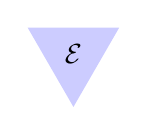
\begin{tikzpicture} [
          triangle/.style = {fill=blue!20, regular polygon, regular polygon sides=3 },
          node rotated/.style = {rotate=180},
          border rotated/.style = {shape border rotate=180}
          ]
          \node[triangle, border rotated] {$\mathcal{E}$};
        \end{tikzpicture}\\
        $A$ true 
      \end{tabular},
      then
      \begin{tabular}{c}
        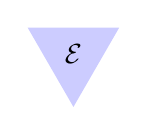
\begin{tikzpicture} [
          triangle/.style = {fill=blue!20, regular polygon, regular polygon sides=3 },
          node rotated/.style = {rotate=180},
          border rotated/.style = {shape border rotate=180}
          ]
          \node[triangle, border rotated] {$\mathcal{E}$};
        \end{tikzpicture}\\
    $A$ true \\ $\mathcal{D}$ \\ $B$ true
      \end{tabular}
    \end{center}

    Basically, if we have a proof for $A$ true and from $A$ true we
    can show $B$ true, then we have a proof for $B$ true.

    \paragraph{Local Completeness}
    \begin{center}
      \begin{tabular}{c}
        $\alpha$
        \\$A \supset B$ true
      \end{tabular}
      $\implies$
      \AXC{$\alpha$}
      \noLine
      \UIC{$A \supset B$ true}
      \AXC{}
      \RL{u}
      \UIC{$A$ true}
      \RL{$\supset$ E}
      \BIC{$B$ true}
      \RL{$\supset$ I$^u$}
      \UIC{$A \supset B$ true}
      \DP
    \end{center}
    So we can prove $A \supset B$ from $A \supset B$.

    Another form of $\land$ elimination:
    \begin{prooftree}
      \AXC{$A \land B$ true}
      \AXC{}
      \RL{u}
      \UIC{$A$ true}
      \AXC{}
      \RL{v}
      \UIC{$B$ true}
      \noLine
      \BIC{\vdots}
      \noLine
      \UIC{$C$ true}
      \RL{$\land E^{u,v}$}
      \BIC{$C$ true}
    \end{prooftree}
    We could use this new rule and check for local soundness and
    completeness like above.

    Could have unused, floating assumption:
    \begin{prooftree}
      \AXC{}
      \RL{a}
      \UIC{$A$ true}
    \end{prooftree}
    \begin{prooftree}
      \AXC{}
      \RL{u}
      \UIC{$A \land B$}
      \RL{b}
      \UIC{$B$ true}
      \AXC{\vdots}
      \noLine
      \UIC{$A$ true}
      \BIC{$B \land A$ true}
      \RL{$\supset$ I$^u$}
      \UIC{$A \land B \supset B \land A$ true}
    \end{prooftree}
    \subsection{Disjunction}
    Intro-Rules:
    \begin{prooftree}
      \AXC{$A$ true}
      \RL{$\lor$ I$_l$}
      \UIC{$A \lor B$ true}
    \end{prooftree}
    \begin{prooftree}
      \AXC{$B$ true}
      \RL{$\lor$ I$_r$}
      \UIC{$A \lor B$ true}
    \end{prooftree}
    Might be tempted to make the following rule:
    \begin{prooftree}
      \AXC{$B$ true}
      \RL{$\lor$ I$_r$}
      \UIC{$A \lor B$ true}
      \RL{?}
      \UIC{$A$ true}
    \end{prooftree}
    This is locally unsound! Got information we didn't start with.

    We also cannot introduce:
    \begin{prooftree}
      \AXC{$A \lor B$}
      \UIC{$\neg A \supset B$ true}
    \end{prooftree}
    This violates our principle of modularity, as we don't want to
    refer to a different kind of connective.

    Our elimination rule:
    \begin{prooftree}
      \AXC{$A \lor B$ true}
      \AXC{}
      \RL{u}
      \UIC{$A$ true}
      \noLine
      \UIC{\vdots}
      \noLine
      \UIC{$C$ true}
      \AXC{}
      \RL{v}
      \UIC{$B$ true}
      \noLine
      \UIC{\vdots}
      \noLine
      \UIC{$C$ true}
      \RL{$\lor$ E$^{u,v}$}
      \TIC{$C$ true}
    \end{prooftree}
    \paragraph{Example}
    \begin{prooftree}
      \AXC{}
      \RL{u}
      \UIC{$A \lor (B \land C)$ true}
      \AXC{}
      \RL{a}
      \UIC{$A$ true}
      \RL{$\lor$ I$_l$}
      \UIC{$A \lor C$ true}
      \AXC{}
      \RL{b}
      \UIC{$B \land C$ true}
      \RL{$\land$ E$_l$}
      \UIC{$A \lor B$ true}
      \UIC{$B$ true}
      \RL{$\lor$ I$_r$}
      \RL{$\lor$ E}
      \TIC{$A \lor B$ true}
      \AXC{\vdots}
      \noLine
      \UIC{$A \lor C$ true} % Same proof as other thing (almost)
      \RL{$\lor$ I}
      \BIC{$(A \lor B)\land (A \lor C)$}
      \RL{$\supset$ I}
      \UIC{$(A \lor (B \land C))\supset (A \lor B)\land (A \lor C)$}
    \end{prooftree}
    \section{01/15/19}
    Recall: We defined $\neg A$ as $A \supset \perp$. But, there are
    other ways you can introduce (define) negation.
    \subsection{Negation}
    \begin{prooftree}
      \AXC{}
      \RL{u}
      \UIC{$A$ true}
      \noLine
      \UIC{\vdots}
      \noLine
      \UIC{$p$ true}
      \RL{$\neg$ I$^{u,p}$}
      \UIC{$\neg A$ true}
    \end{prooftree}
    If we can prove any parameter $p$ from $A$ true, then $\neg A$ is
    true. This discharges the assumption $u$ and $p$.
    \begin{prooftree}
      \AXC{$\neg A$ true}
      \AXC{$A$ true}
      \RL{$\neg$ E}
      \BIC{$C$ true}
    \end{prooftree}
    For these new rules, as usual, we want to prove that they are
    locally sound and complete. In general, for local soundness, you
    want to introduce the rule and then eliminate it and show that
    you've learned nothing new.
    \paragraph{Local Soundness}
    \begin{center}
      \AXC{}
      \RL{u}
      \UIC{$A$ true}
      \noLine
      \UIC{$D$}
      \noLine
      \UIC{$p$ true}
      \RL{$\neg$ I$^{p,u}$}
      \UIC{$\neg A$ true}
      \AXC{$\mathcal{E}$}
      \noLine
      \UIC{$A$ true}
      \RL{$\neg$ E}
      \BIC{$C$ true}
      \DP
      $\implies$
      \begin{tabular}{c}
        $ [\mathcal{E}/u, C/p]D$
        \\ $C$ true
      \end{tabular}
    \end{center}
    \paragraph{Local Completeness}
    \begin{center}
      \begin{tabular}{c}
        $\mathcal{D}$
        \\ $\neg A$ true
      \end{tabular}
      $\implies$
      \AXC{$\mathcal{D}$}
      \noLine
      \UIC{$\neg A$ true}
      \AXC{}
      \RL{u}
      \UIC{$A$ true}
      \RL{$\neg$ E}
      \BIC{$p$ true}
      \RL{$\neg$ I$^{p,u}$}
      \UIC{$\neg A$ true}
      \DP
    \end{center}
    \subsection{Classical Reasoning}
    Basic idea behind proof by contradiction, you assume $\neg A$,
    arrive at a contradiction and then you can prove $A$ true.

    \begin{prooftree}
      \AXC{}
      \RL{u}
      \UIC{$\neg A$ true}
      \noLine
      \UIC{\vdots}
      \noLine
      \UIC{$p$ true}
      \RL{$C^{u,p}$}
      \UIC{$A$ true}
    \end{prooftree}
    where $C^{u,p}$ means a proof by contradiction under $u$ and $p$.
    \paragraph{Law of Excluded Middle}
    Want to show $\neg A \lor A$ is true for all $A$.
    \begin{prooftree}
      
      \AXC{}
      \RL{u}
      \UIC{$\neg (\neg A \lor A)$ true}

      \AXC{}
      \RL{v}
      \UIC{$\neg A$}
      \RL{$\lor$ I$_l$}
      \UIC{$\neg A \lor A$}
      
      \RL{$\neg$ E}
      \BIC{$p$ true}
      \RL{$C^{v,p}$}
      \UIC{$A$}
      \RL{$\lor$ I$_r$}
      \UIC{$\neg A \lor A$}
      
      \AXC{}
      \RL{u}
      \UIC{$\neg (\neg A \lor A)$ true}
      \RL{$\neg$ E}
      
      \BIC{$q$ true}
      \RL{$C^{u,q}$}
      \UIC{$\neg A \lor A$}
    \end{prooftree}
    \paragraph{Law of Excluded Middle and more examples in tutch}
    \lstinputlisting{lem.tut}
    \subparagraph{Output}
    \lstinputlisting{lem.tut.output}
    \subsection{NAND}
    $A \overline{\land} B \equiv \neg (A \land B)$

    Showing this introduction rule is often a midterm question. Often,
    people make the mistake of using $A \land B$, but we cannot
    introduce other connectives, make sure $A$ and $B$ are separate.
    \begin{prooftree}
      \AXC{}
      \RL{u}
      \UIC{$A$ true}
      \AXC{}
      \RL{v}
      \UIC{$B$ true}
      \noLine
      \BIC{\vdots}
      \noLine
      \UIC{$p$ true}
      \RL{$\overline{\land}$ I}
      \UIC{$A \overline{\land} B$ true}
    \end{prooftree}
    \begin{prooftree}
      \AXC{$A$ true}
      \AXC{$B$ true}
      \AXC{$A \overline{\land} B$ true}
      \RL{$\overline{\land}$ E}
      \TIC{$C$ true}
    \end{prooftree}
    \paragraph{Local Soundness}
    Get rid of assumptions by substituting $\mathcal{E}_1,
    \mathcal{E}_2$ and $C$ into $\mathcal{D}$.
    \begin{center}
      \AXC{}
      \RL{u}
      \UIC{$A$ true}
      \AXC{}
      \RL{v}
      \UIC{$B$ true}
      \noLine
      \BIC{$\mathcal{D}$}
      \noLine
      \UIC{$p$ true}
      \RL{$\overline{\land}$ I$^{u,v,p}$}
      \UIC{$A \overline{\land} B$ true}
      \AXC{$\mathcal{E}_1$}
      \noLine
      \UIC{$A$ true}
      \AXC{$\mathcal{E}_2$}
      \noLine
      \UIC{$B$ true}
      \TIC{$C$ true}
      \DP
      $\implies$
      \begin{tabular}{c}
        $[\mathcal{E}_1/u, \mathcal{E}_2/v, C/p] \mathcal{D}$
        \\ $C$ true
      \end{tabular}
    \end{center}
    \paragraph{Local Completeness}
    \begin{center}
      \begin{tabular}{c}
        $\mathcal{D}$
        \\ $A \overline{\land} B$
      \end{tabular}
      $\implies$
      \AXC{}
      \RL{u}
      \UIC{$A$ true}
      \AXC{}
      \RL{v}
      \UIC{$B$ true}
      \AXC{$\mathcal{D}$}
      \noLine
      \UIC{$A \overline{\land} B$ true}
      \RL{$\overline{\land}$ E}
      \TIC{$p$ true}
      \RL{$\overline{\land}$ I$^{u,v,p}$}
      \UIC{$A \overline{\land} B$}
      \DP
    \end{center}
    Look for other connectives and do these proofs, as they will
    probably be on the midterm.
    \section{01/17/19}
    \subsection{Context}
    So we've seen several rules so far:
    \begin{prooftree}
      \AXC{}
      \UIC{$T$ true}
    \end{prooftree}
    \begin{prooftree}
      \AXC{$\perp$ true}
      \RL{}
      \UIC{$C$ true}
    \end{prooftree}
    \begin{prooftree}
      \AXC{$A$ true}
      \AXC{$B$ true}
      \RL{$\land$ I}
      \BIC{$A \land B$}
    \end{prooftree}
    \begin{prooftree}
      \AXC{$A \land B$ true}
      \RL{$\land$ E$_l$}
      \UIC{$A$ true}
    \end{prooftree}
    \begin{prooftree}
      \AXC{$A \lor B$ true}
      \AXC{}
      \RL{u}
      \UIC{$A$ true}
      \noLine{}
      \UIC{\vdots}
      \noLine
      \UIC{$C$ true}
      
      \AXC{}
      \RL{v}
      \UIC{$B$}
      \noLine
      \UIC{$\vdots$}
      \noLine
      \UIC{$C$ true}
      \RL{$\lor$ E$^{u,v}$}
      \TIC{$C$ true}
    \end{prooftree}
    We are now going to extend these rules with contexts, which allows
    us to know what we've proved and what assumptions we have at each
    step.

    Instead of $A$ true, we will write $\Gamma \vdash A$ true. This
    means:

    ``A is true in context $\Gamma$.''

    $$\Gamma ::= \cdot \mid \Gamma, u:A \text{ true}$$

    So:
    \begin{center}
      \AXC{}
      \RL{u}
      \UIC{$A$ true}
      \noLine
      \UIC{\vdots}
      \noLine
      \UIC{$B$ true}
      \RL{$\supset$ I$^u$}
      \UIC{$A \supset B$ true}
      \DP
      $\stackrel{+\Gamma}{\longrightarrow}$
      \AXC{$\Gamma,u:A$ true $\vdash B$ true}
      \UIC{$\Gamma \vdash A \supset B$ true}
      \DP
    \end{center}
    \begin{prooftree}
      \AXC{}
      \UIC{$\Gamma \vdash T$ true}
    \end{prooftree}
    \begin{prooftree}
      \AXC{$\Gamma \vdash \perp$ true}
      \RL{}
      \UIC{$\Gamma \vdash C$ true}
    \end{prooftree}
    \begin{prooftree}
      \AXC{$\Gamma \vdash A$ true}
      \AXC{$\Gamma \vdash B$ true}
      \RL{$\land$ I}
      \BIC{$\Gamma \vdash A \land B$}
    \end{prooftree}
    \begin{prooftree}
      \AXC{$\Gamma \vdash A \land B$ true}
      \RL{$\land$ E$_l$}
      \UIC{$\Gamma \vdash A$ true}
    \end{prooftree}
    \begin{prooftree}
      \AXC{$\Gamma \vdash A \lor B$ true}
      \AXC{$\Gamma,u: A $ true $\vdash C$}
      \AXC{$\Gamma,v: B $ true $\vdash C$}
      \RL{$\lor$ E$^{u,v}$}
      \TIC{$\Gamma\vdash C$ true}
    \end{prooftree}
    For something to be derived from a context:
    \begin{prooftree}
      \AXC{$u: A$ true $\in \Gamma$}
      \RL{H}
      \UIC{$\Gamma \vdash A$ true}
    \end{prooftree}
    \paragraph{Example}
    \begin{prooftree}
      \AXC{$A \in \Gamma, A, B$}
      \RL{H}
      \UIC{$\Gamma, A, B \vdash$ A}
      \AXC{$B \in \Gamma, A, B$}
      \RL{$H$}
      \UIC{$\Gamma, A, B \vdash$ B}
      
      \RL{$\land$ I}
      \BIC{$\Gamma, u: A$ true, $B$ true $\vdash A \land B$}
      \RL{$\supset$ I}
      \UIC{$\Gamma,u:A$ true $\vdash B \supset A \land B$}
      \RL{$\supset$ I}
      \UIC{$\Gamma \vdash A \supset B \supset A \land B$}
    \end{prooftree}
    \subsection{The Curry-Howard Correspondence}
    We can see that natural deduction is the same as
    functional programming:
    \\
    \begin{tabular}{c c}
      Logic & Types
      \\ \hline $\perp$ & unit
      \\ $A \land B$ & $A \times B$
      \\ $A \lor B$ & $A + B$
      \\ $A \supset B$ & $A \implies B$
      \\ $\perp$ & $\emptyset$
      \\ proofs & programs
      \\ checking a proof & type checker
    \end{tabular}
    \\
    
    $\emptyset$ is the empty type. There is no proof for $\perp$,
    which is why there is no program for $\emptyset$, the two sides
    are equivalent.

    Proof terms capture the structure of a derivation.

    \begin{prooftree}
      \AXC{}
      \RL{H}
      \UIC{$\Gamma,x:A,y:B\vdash x:A$}
      \AXC{}
      \RL{H}
      \UIC{$\Gamma,x:A,y:B\vdash y:B$}
      \RL{$\times$ I}
      \BIC{$\Gamma,x:A,y:B \vdash (x,y): A \times B$}
      \RL{$\implies$ I$^y$}
      \UIC{$\Gamma,x:A \vdash fn\ y \implies (x,y): B \implies A \times
        B$}
      \RL{$\implies$ I$^x$}
      \UIC{$\Gamma \vdash fn\ x \implies fn\ y \implies (x,y) : A \implies B \implies A \times B$}
    \end{prooftree}

    $\Gamma \vdash M : A$ means:\\
    ``M is a proof term (program) for proposition (of type) A.''
    \subsection{Proof Terms}
    Let's upgrade the rules we mentioned earlier to types:
    \begin{prooftree}
      \AXC{}
      \UIC{$\Gamma \vdash () : unit$}
    \end{prooftree}
    \begin{prooftree}
      \AXC{$\Gamma \vdash M: \emptyset$}
      \RL{}
      \UIC{$\Gamma \vdash abort\ M : C$}
    \end{prooftree}
    \begin{prooftree}
      \AXC{$\Gamma \vdash M_1: A$ true}
      \AXC{$\Gamma \vdash M_2: B$ true}
      \RL{$\times$ I}
      \BIC{$\Gamma \vdash (M_1, M_2)\ A\ B$ true}
    \end{prooftree}
    \begin{prooftree}
      \AXC{$\Gamma \vdash M: A \times B$}
      \RL{$\times$ E$_l$}
      \UIC{$\Gamma \vdash fst\ M: A$}
    \end{prooftree}
    \begin{prooftree}
      \AXC{$\Gamma \vdash M: A \times B$}
      \RL{$\times$ E$_r$}
      \UIC{$\Gamma \vdash snd\ M: B$}
    \end{prooftree}
    \begin{prooftree}
      \AXC{$\Gamma \vdash M: A + B$ true}
      \AXC{$\Gamma,u: A \vdash N_1:C$}
      \AXC{$\Gamma,v: B \vdash N_2:C$}
      \RL{$+$ E}
      \TIC{$\Gamma\vdash $ case $M$ of}
      \noLine
      \UIC{inl $u \implies N_1$}
      \noLine
      \UIC{inr $v \implies N_2$}
    \end{prooftree}
    (Where inl is inject left and inr is inject right) Note that this
    is pattern matching!
    \begin{prooftree}
      \AXC{$\Gamma, x:A \vdash M:B$}
      \UIC{$\Gamma \vdash (fn\ x \implies M):A \implies B$}
    \end{prooftree}
    \begin{prooftree}
      \AXC{$\Gamma \vdash M : A$}
      \RL{$+$ I$_l$}
      \UIC{$\Gamma \vdash inl \ M: A + B$}
    \end{prooftree}
    \begin{prooftree}
      \AXC{$\Gamma \vdash M : B$}
      \RL{$+$ I$_r$}
      \UIC{$\Gamma \vdash inr \ M: A + B$}
    \end{prooftree}
    \begin{prooftree}
      \AXC{$\Gamma \vdash M : A \implies B$}
      \AXC{$\Gamma \vdash N : A$}
      \BIC{$\Gamma \vdash M\_N: B$}
    \end{prooftree}
    where $\_$ is a space.
    \paragraph{Example}
    We did this on Tuesday, now we'll see it with proof terms.
    \begin{prooftree}
      \AXC{}
      \RL{H}
      \UIC{$\Gamma, x : A \times B \vdash x : A \times B$}
      \RL{$\times$ E}
      \UIC{$\Gamma, x: A \times B \vdash snd\ x : B$}
      
      \AXC{}
      \RL{H}
      \UIC{$\Gamma, x : A \times B \vdash x : A \times B$}
      \RL{$\times$ E}
      \UIC{$\Gamma, x: A \times B \vdash fst\ x : A$}
      \RL{$\times$ I}
      
      \BIC{$\Gamma, x: A \times B \vdash (snd\ x, fst\ x) : B \times
        A$}
      \RL{$\implies$ I}
      \UIC{$\Gamma \vdash fn\ x \implies (snd\ x, fst\ x) : A \times B \implies B \times A$}
    \end{prooftree}
    \paragraph{Tutch Examples}
    \lstinputlisting[breaklines=true]{proofterms.tut}
    \section{01/22/19}
    \subsection{Metatheory}
    Proving things (properties) about a given theory, this will
    eventually lead us to completeness.

    So far, we've seen:
    \paragraph{Propositions/Types} $A,B:=T \mid \perp \mid A \supset B \mid A
    \land B \mid A \lor B$

    \paragraph{Proof Terms} $M,N := \langle \rangle \mid abort^{A}\ M
    \mid \underbrace{\lambda x: A.M}_{fn\ x \implies M} \mid M \ N$

    \begin{prooftree}
      \AXC{$M : \perp$}
      \UIC{$abort^{A}\ M : A$}
    \end{prooftree}

    Note that: $M : A$ means: Term $M$ has type $A$ or $M$ is a proof
    witness for the proposition $A$

    Types that have one type are sometimes just called singleton
    types.

    Earlier we saw:
    \begin{prooftree}
      \AXC{}
      \RL{$u_1$}
      \UIC{$A_1$ true}
      \UIC{$\ddots$}

      \AXC{\ldots}

      \AXC{}
      \RL{$u_n$}
      \UIC{$A_n$ true}
      \UIC{$\ddots$}

      \TIC{$C$ true}
    \end{prooftree}
    More compactly: Context $\Gamma := \cdot \mid T, A$ true

    $$\Gamma \underbrace{\vdash}_{\text{turnstyle}} C \text{ true}$$

    \paragraph{Reminder about Contexts}
    Context $\Gamma := \cdot \mid \Gamma, x: A$
    \begin{prooftree}
      \AXC{$\Gamma \vdash M : \perp$}
      \UIC{$\Gamma \vdash abort^{A}\ M : A$}
    \end{prooftree}
    \begin{prooftree}
      \AXC{$\Gamma,x:A \vdash M : B$}
      \UIC{$\Gamma \vdash \lambda x:A.M: A \supset B$}
    \end{prooftree}
    \begin{prooftree}
      \AXC{$\Gamma \vdash M : A \supset B$}
      \AXC{$\Gamma \vdash N : A$}
      \BIC{$\Gamma \vdash M\ N:B$}
    \end{prooftree}
    \begin{prooftree}
      \AXC{$x : A \in \Gamma$}
      \UIC{$\Gamma \vdash x : A$}
    \end{prooftree}
    \begin{prooftree}
      \AXC{$\Gamma \vdash M : A$}
      \AXC{$\Gamma \vdash N : B$}
      \BIC{$\Gamma \vdash \langle M, N \rangle : A \land B$}
    \end{prooftree}
    \begin{prooftree}
      \AXC{$\Gamma \vdash M : A \land B$}
      \UIC{$\Gamma \vdash fst \ M : A$}
    \end{prooftree}
    Note that, some may be inclined to make $A \land B$ have a type of
    some pair, like $(M,N)$, but we don't want to limit ourselves to a
    pair (we also don't yet know it's a pair), so we cannot make it a
    pair right off the bat.
    \begin{prooftree}
      \AXC{$\Gamma \vdash M : A \land B$}
      \UIC{$\Gamma \vdash snd \ M : B$}
    \end{prooftree}
    What would we like to compute with these rules?

    General form: $M \implies M'$, Term $M$ reduces to $M'$.
    \\ $fst\ \langle M, N \rangle \implies M$
    \\ $snd\ \langle M, N \rangle \implies N$

    So we can now show things like local soundness:
    \begin{center}
      \AXC{$\mathcal{D}_1$}
      \noLine
      \UIC{$\Gamma \vdash M : A$}
      \AXC{$\mathcal{D}_2$}
      \noLine
      \UIC{$\Gamma \vdash N : B$}
      \RL{$\land$ I}
      \BIC{$\Gamma \vdash \langle M, N \rangle : A \land B$}
      \RL{$\land$ E$_l$}
      \UIC{$\Gamma \vdash fst \ \langle M, N \rangle : A$}
      \DP
      $\implies$
      \begin{tabular}{c}
        $\mathcal{D}_1$
        \\ $M : A$
      \end{tabular}
    \end{center}
    Local Soundness here corresponds to Subject Reduction/Type
    Preservation.

    We've essentially proved that if we start with something well
    typed (of type $A$), we end up with something that is still well
    typed, we can show that our program is type \textbf{safe}.

    Now if we have a function:

    $(\lambda x : A . M) N \implies [N/x] M$
    \paragraph{Simple Program}
    \begin{align*}
      & fst \ ((\lambda x . \lambda y . \langle x , y \rangle) \langle \rangle \langle \rangle)
      \\ \implies & fst \ \langle \langle \rangle, \langle \rangle \rangle
      \\ \implies & \langle \rangle : T
    \end{align*}
    The type of this program is unit, because we have stated earlier
    that the type we start with is the type we end with. How do we
    know the first line is of type unit?
    \begin{prooftree}

      \AXC{}
      \RL{var}
      \UIC{$x:T, y:T \vdash x:T$}
      
      \AXC{}
      \RL{var}
      \UIC{$x:T, y:T \vdash y:T$}

      \RL{$\land$ I}
      \BIC{$x: T, y:T \vdash \langle x,y \rangle : T \land T$}
      \UIC{$x:T \vdash \lambda y:T \langle x,y \rangle : T \supset (T
        \land T)$}
      \RL{$\supset$ I}
      \UIC{$\lambda x: T \lambda . y: T \langle x,y \rangle : T \supset
        T \supset (T \land T)$}
      
      \AXC{}
      \RL{$T$ I}
      \UIC{$\langle \rangle$ : T}
      
      \RL{$\supset$ E}
      \BIC{$(\lambda x : T \lambda . y: T \langle x,y \rangle)$ : $\langle \rangle$}
      
      \AXC{}
      \RL{$T$ I}
      \UIC{$\langle \rangle$ : T}
      
      \BIC{$((\lambda x:T . \lambda y: T \langle x,y \rangle) \langle
        \rangle) \langle \rangle$ : }
      \RL{$\land$ E$_l$}
      \UIC{$fst\ (\lambda x : T . \lambda y : T \langle x,y \rangle)
        \langle \rangle \langle \rangle$ : }
    \end{prooftree}

    The following is a theorem we are not going to prove:

    If $\Gamma \vdash M : A$ and $M \implies M'$ then $\Gamma \vdash
    M': A$
    
    If $\Gamma \vdash M' : A$ and $M \implies M'$ then $\Gamma \vdash
    M: A$
    \subsection{Congruence Rules}
    We can go into functions. This strategy is non-deterministic (will
    this terminate? Yes, but it is not obvious how to prove it. This
    is a metatheoretic property)
    \begin{prooftree}
      \AXC{$M \implies M'$}
      \UIC{$fst \ M \implies fst \ M'$}
    \end{prooftree}
    \begin{prooftree}
      \AXC{$M \implies M'$}
      \UIC{$snd \ M \implies snd \ M'$}
    \end{prooftree}
    \begin{prooftree}
      \AXC{$M \implies M'$}
      \UIC{$M \ N \implies M' \ N$}
    \end{prooftree}
    \begin{prooftree}
      \AXC{$N \implies N'$}
      \UIC{$M \ N \implies M \ N'$}
    \end{prooftree}
    \begin{prooftree}
      \AXC{$M \implies M'$}
      \UIC{$\lambda x:A.M \implies \lambda x : A.M'$}
    \end{prooftree}
    \paragraph{Syntactic Equality} is important because we want to
    introduce substitution.
    \\\begin{tabular}{l l}
      $\lambda x.x = \lambda y.y$ & \text{(the name of a bound var
                                  does not matter)}
        \\ $\lambda x . \lambda y. x \neq \lambda x . \lambda y . y$
        \\ $\lambda x. \lambda y. x = \lambda x' . \lambda y . x'$ & These are the same because $x$ has the same binding site as $x'$
      \end{tabular}
      \\
    Terms that only differ in the names of the bound variables are
    considered equal. This is defined as
    $\alpha$-renaming. Capture-avoiding substitution.

    Note in the following expression, $x$ is new (``fresh''). We
    cannot have two variables with the same name, if this was the
    case, we'd have to rename $x$. 

    \begin{prooftree}
      \AXC{$\Gamma, x: A \vdash M : B$}
      \UIC{$\Gamma \vdash \lambda x : A . M : A \supset B$}
    \end{prooftree}

    Otherwise a rule such as the following would not give you
    a unique type.
    \begin{prooftree}
      \AXC{$x:A \in \Gamma$}
      \UIC{$\Gamma \vdash x : A$}
    \end{prooftree}
    \paragraph{Example of substitution} What does this mean?
    \\ $[u/w] (\lambda u.w u) \neq \lambda u. u u$
    \\ You cannot introduce a new variable with the same name as an
    existing one, this will have completely different meaning than you
    intended.
    \\ Solution: $[u/w](\lambda y: w
    u)\stackrel{\alpha}{=}[u/w](\lambda u'. w u') = \lambda u'. u u'$

    Let's assume that $u : T \supset A$.
    \\ $[u/w](\underbrace{\lambda u : T. \ w \ u}_{\text{well-typed, $T
        \supset A$}}) = \lambda u : T. \ \underline{u} \ u$? This is
    ill-typed!
    \subsection{Restatement of Definitions Using Context}
    \paragraph{Weakening} If $\Gamma \vdash M:A$ then $\Gamma, \Gamma'
    \vdash M:A$
    \paragraph{Substitution} If $\Gamma, x : A , \Gamma' \vdash M : B$
    and $\Gamma \vdash N : A$ then $\Gamma, \Gamma' \vdash [N/x] M : B$

    How do we prove this? Proof by structural on $\Gamma, x: A,
    \Gamma' \vdash M : B$

    First we must consider each rule that could have been used to derive
    $M : B$.

    Base case would be T, trivially true because there is nothing to
    substitute.

    \subparagraph{Definition of substitution}
    ~\\$[N/x]M = M'$, $[N/x] x = N$. Replace the "free" occurence of
    $x$ in $M$ with $N$
    
    \subparagraph{Case}
    \AXC{$\mathcal{D}'$}
    \noLine
    \UIC{$\Gamma, x:A, \Gamma' \vdash M : C \land D$}
    \RL{$\land$ E$_l$}
    \UIC{$\Gamma, x:A,\Gamma' \vdash fst\ M : C$}
    \DP
    \\ $\Gamma, \Gamma ' \vdash [N/x] M : C\land D$ by IH
    \\ $\Gamma, \Gamma ' \vdash fst\ ([N/x]M) : C$ by $\land$E$_l$
    \\$\Gamma, \Gamma' \vdash [N/x](fst \ M) : C$ by definition of substitution
    \subparagraph{Case}
    \AXC{$\mathcal{D}_1$}
    \noLine
    \UIC{$\Gamma, x:A, \Gamma' \vdash M_1 : D \supset C $}
    
    \AXC{$\mathcal{D}_2$}
    \noLine
    \UIC{$\Gamma, x:A, \Gamma' \vdash M_2 : D$}
    \RL{$\supset$ E}
    \BIC{$\Gamma, x:A,\Gamma' \vdash M_1 \ M_2 : C$}
    \DP
    \\ $\Gamma, \Gamma ' \vdash [N/x] M_1 : D \supset C$ by IH ($\mathcal{D}_1$)
    \\ $\Gamma, \Gamma ' \vdash [N/x] M_2 : D$ by IH ($\mathcal{D}_2$)
    \\$\Gamma, \Gamma' \vdash [N/x]M_1 \ [N/x]M_2 : C$ by $\supset$ E
    \\ $\Gamma, \Gamma' \vdash [N/x](M_1\ M_2) : C$

    The more interesting case is with variables:
    \subparagraph{Case}
    \AXC{$x: A \in (\Gamma, x : A, \Gamma')$}
    
    \UIC{$\Gamma, x : A, \Gamma' \vdash x : A$}
    \DP
    \\ $\Gamma \vdash N:A$ by assumption
    \\ $\Gamma, \Gamma' \vdash N : A$ by weakening
    \\ $\Gamma, \Gamma' \vdash [N/x]x : A$ by substitution definition
    \subparagraph{Case}
    \AXC{$y: B \in (\Gamma, x : A, \Gamma')$}
    \AXC{$x \neq y$}
    
    \BIC{$\Gamma, x : A, \Gamma' \vdash y : B$}
    \DP
    \\ $y:B \in (\Gamma, \Gamma')$
    \\ $\Gamma, \Gamma' \vdash y : B$ by variable
    \subparagraph{Case}
    \AXC{$\Gamma, x : A, \Gamma', y:B \vdash M:C$}
    
    \UIC{$\Gamma, x : A, \Gamma' \vdash \lambda y : B. M:B\supset C$}
    \DP
    \\ $\Gamma, \Gamma', y:B \vdash [N/x] M:C$ by IH.
    \\ $\Gamma, \Gamma', \lambda y : B . [N/x] M: B \supset C$ by $\supset$ I 
    \\ $\Gamma \vdash N : A$ by assumption (i.e any var in $N$ is in
    $\Gamma$). $y$ does not occur in $N$
    \\ $\Gamma, \Gamma ' \vdash [N/x] (\lambda y:B.M) : B \supset C$
    by substitution definition
    \section{01/24/19}
    \subsection{More on Proof Terms}
    Last class we saw:
    \\ Prop/Types $A,B:= T \mid \perp \mid A \land B \mid A \supset B
    \mid A \lor B$
    \\ Terms $M,N := \langle  \rangle \mid abort^c \ M \mid \langle
    M,N \rangle \mid fst\ M \mid snd \ M \mid \lambda x . A . M \mid M
    \ N \mid inl^B \ M \mid inr^A \ B \mid (case \ M \ of \ inl \ x
    \implies N_1 \mid inr\ y \implies N_2)$

    We can think of $M:A$ iff $A$ true.
    \paragraph{Warm-up}
    \begin{center}
      \begin{tabular}{l l}
        \textbf{Program} & \textbf{Proposition}
        \\ $\lambda x : A . \lambda y: B. \langle x,y \rangle$ & $A \supset B \supset (A \land B)$
        \\ $\lambda x : A \supset B  \land B \supset C$ & $(A \subset B \land B \supset C) \supset A \supset C$
        \\ ~\hspace{5 pt} $\lambda y: A.(snd\ x)\underbrace{(\underbrace{(fst\ x)}_{A \supset B} y)}_{B}$
        \\ $\lambda x : A \lor B. \lambda y: C$& $(A \lor B) \supset C \supset (B \lor A) \land C$
        \\ ~\hspace{5 pt} $\langle case \ of \ inl \ a \implies inr\ a \mid inr\ b \implies inl\ b,y  \rangle$
      \end{tabular}
    \end{center}
      \paragraph{Reminder}
      \begin{tabular}{l l}
        Prop & Type
        \\ $T$ & unit
        \\ $A \land B$ & $A * B$
        \\ $A \supset B$ & $A \rightarrow B$
        \\ $ A \lor B$ & $A + B$
      \end{tabular}
      The $+$ is usually hidden in programming languages,
      i.e. \texttt{type int\_or\_string = Int of int | Str of string}
      is actually \texttt{Int + String}.
    \begin{center}
      \begin{tabular}{l l}
        \textbf{Proposition} & \textbf{Program}
        \\ $A \supset A$ (has many programs) & $\lambda x:A.x$ \hspace{10 pt}normal/``canonical form''
        \\ Programs on the right are syntactically different & $\lambda x : A . (\lambda y: A . y) x$
        \\ & $\lambda x : A . fst ((\lambda y:A \land A . y) \langle x,x \rangle)$
      \end{tabular}
    \end{center}
    We hope that all of the functions on the right can reduce to the
    normal form.

    If $\Gamma \vdash M : A$ and $M \implies M'$ then $\Gamma \vdash
    M' : A$ \} Subject Reduction/Type Preservation

    By induction (case analysis) on $M \implies M'$
    \subparagraph{Case} $fst \langle M,N \rangle \implies M$
    \\\begin{tabular}{l l}
    $\Gamma \vdash fst\ \langle M,N \rangle : A$ & by assumption
    \\ $\Gamma \vdash \langle M,N \rangle : A \land B$ & by \underline{inversion} on
    $\land$ E$_l$
    \end{tabular}

    Note the inversion rule tells us:
    \begin{prooftree}
      \AXC{$M : A \land B$}
      \RL{$\land$ E$_l$}
      \UIC{$fst\ M : A$}
    \end{prooftree}
    Inversion Lemma: If $fst\ M : A$ then $M:A \land B$. This is
    obvious in this system because there is only one rule. If there
    was another rule that we could use, then we'd have to prove that
    it came from this inversion rule.
    \\\begin{tabular}{l l}
    $\Gamma \vdash M : A$ & by \underline{inversion} of $\land I$
    \end{tabular}

    The concept of \underline{inversion} is very important, we want to
    know where the term comes from.
    \subparagraph{Case} $(\lambda x : A.M) N \implies [N/x] M$
    \\\begin{tabular}{l l}
    $\Gamma \vdash (\lambda x : A . M) N : B$ & by assumption
    \\ $\Gamma \vdash \lambda x: A.M : A \supset B,\ \Gamma \vdash N :
    A$ & by inversion on $\supset$ E
    \\ $\Gamma, x : A \vdash M : B$ & by inversion on $\supset$ I
    \\ $\Gamma \vdash [N/x]M:B$ & by substitution lemma (on above line
    and $\Gamma \vdash N:A$)
    \end{tabular}
    \subparagraph{Case} $case\ (inl^B \ M) \ of \ inl\ x \implies N_1
    \mid inr\ y \implies N_2 \implies [M/x] N_1$
    \\\begin{tabular}{l l}
    $\Gamma \vdash case\ (inl^B \ M) \ of \ inl\ x \implies N_1
        \mid inr\ y \implies N_2 : C $ & by assumption
        \\ $\Gamma \vdash inl^B \ M : A \lor B$ & by inversion $\lor$ E
        \\ $\Gamma, x:A \vdash N_1 : C$
        \\ $\Gamma, x:B \vdash N_2 : C$
        \\ $\Gamma \vdash M.A : C$ & by inversion $\lor$ I$_l$
        \\ $\Gamma \vdash [M/x]N_1 : C$ & by substitution
      \end{tabular}
      \subparagraph{Case} \AXC{$M_1 \implies M'$}
      \UIC{$M_1 \ M_2 \implies M_1' M_2$}
      \DP
      \\
      \begin{tabular}{l l}
        $\Gamma \vdash M_1 \ M_2 : B$& by assumption
        \\ $\Gamma \vdash M_1 : A \supset B$ and $\Gamma \vdash M_2 : A$ & by inversion $\supset$E
        \\ $\Gamma \vdash M_1' : A \supset B$ & by IH
        \\ $\Gamma \vdash M_1' M_1 : B$ & by $\supset$ E
      \end{tabular}
      The last step is forward reasoning instead of backward reasoning
      with inversions. Basically show what your case gives you and
      then apply IH to get what you want.
      \subparagraph{Case}
      \AXC{$M \implies M'$}
      \UIC{$\lambda x : A.M \implies \lambda x: A.M'$}
      \DP
      \\\begin{tabular}{l l}
        $\Gamma \vdash \lambda x : A . M : A \supset B$& by assumption
          \\ $\Gamma, x : A \vdash M:B$ & by inversion on $\supset$ I
          \\ $\Gamma, x:A \vdash M' : B$ & by IH
          \\ $\Gamma \vdash \lambda x : A . M' : A \supset B$ & by $\supset$ I
        \end{tabular}

      Note that in trying to reduce $fst\ ((\lambda y:A \land A. y)
      \langle x,x \rangle)$, we will need to step twice:
      \\ $\implies \lambda x : A . fst \langle x,x \rangle$
      \\ $\implies \lambda x : A . x$
      \\ But so far we are only stepping once.
      \paragraph{Can we prove the opposite?}
      If $\Gamma \vdash M' : A$ and $M \implies M'$ then $\Gamma
      \vdash M : A$
      \subparagraph{Case} $fst \langle M,N \rangle \implies M$
      \\\begin{tabular}{l l}
          $\Gamma \vdash M :A$& by assumption
          \\ $\Gamma \vdash N : B$ & How to show this?
          \\ $\Gamma \vdash \langle M,N \rangle : A \land B$
          \\ $\Gamma \vdash fst \ \langle M,N \rangle : A$ & To show
        \end{tabular}
\\        Cannot prove this syntactically right now.
        \paragraph{Multi Step} Want to step multiple times. $M
        \implies^* M'$, meaning $M$ steps in more than one step.
        \begin{prooftree}
          \AXC{}
          \RL{refl(ectivity)}
          \UIC{$M \implies^* M$}
        \end{prooftree}
        \begin{prooftree}
          \AXC{$M \implies^* K$}
          \AXC{$K \implies^* N$}
          \RL{Trans(itivity)}
          \BIC{$M \implies^* N$}
        \end{prooftree}
        \begin{prooftree}
          \AXC{$M \implies N$}
          \RL{one-step}
          \UIC{$M \implies^* N$}
        \end{prooftree}
        \subsection{Normal Form}
        What is a normal form when no reduction is possible anymore?
        \\ $\lambda :A \supset B.\lambda y : A . x \ y$ is a normal
        form
        \\ So is $\lambda x : (A \supset A)\supset C . x \underbrace{(\lambda y: A
          . y)}_{A \supset A}$
        \\ Basically, you can no longer reduce the expression.
        \paragraph{Normal Form} $m,n : = \lambda x:A.m \mid r$
        \paragraph{Neutral Form} $r : = x \mid r \ m \mid fst\ r \mid
        snd\ r$
        \paragraph{Questions}
        \begin{enumerate}
        \item Can we always reach a normal form? (Does reduction
          terminate?)
        \item Can we change the proof that correspond to the normal
          forms? ``Normal Proof'' (without any detours)
        \item Is there a unique normal form that can be computed?
          \\ If $M \implies^* N_1$ and $M \implies^* N_2$ then $N_1 = N_2$
        \end{enumerate}
        Will look at 1 and 2 before the midterm.
        \section{01/29/19}
        \subsection{First-order Logic}
        Reason about domains (nat, list, trees, programs, \ldots)

        How to reason in \underline{general}
        $$\forall x : \underbrace{\tau}_{\text{domain}} : A(x)\ true$$

        \underline{For all} elements in domain $\tau$, $A(x)$ is true.
        \begin{align*}
          & \forall x : nat\ even(x) \supset \neg odd(x)
          \\ & \forall x : \tau:\forall y:\tau P(x) \supset P(y)
          \\ & (\forall x: \tau . P(x)) \supset \exists x:\tau. P(x)
        \end{align*}
        We define truth of a proposition for all possible domains.
        \paragraph{Well-Formedness:} $A$ wf
        \begin{prooftree}
          \AXC{$\tau$ type ($\tau$ itself is wf)}
          \AXC{}
          \UIC{$x : \tau$}
          \noLine
          \UIC{\vdots}
          \noLine
          \UIC{$A(x)$ wf}
          \BIC{$\forall x : \tau. A(x)$ wf}
        \end{prooftree}
        \begin{prooftree}
          \AXC{$t_1:\tau$}
          \AXC{\ldots}
          \AXC{$t_n:\tau$}
          \TIC{$P(t_1,\ldots,t_n)$ wf}
        \end{prooftree}
        $\forall x: nat \ even \ y \supset even (x)$, this is not well
        formed!

        What is a type? What are its elements?

        \begin{tabular}{l l l}
          nat type& \AXC{}\UIC{$z$:nat}\DP& \AXC{$n$:nat}\UIC{$succ\ n$:nat}\DP
          \\ nat\_list type & \AXC{}\UIC{$nil$:nat\_list}\DP & \AXC{$n$:nat}\AXC{$t$:nat\_list}\BIC{$cons(n,t)$:nat\_list}\DP
        \end{tabular}

        Prop. $A,B:= T \mid \perp \mid A \land B \mid \forall
        x:\tau. A(x)$
        \\ Terms $t:= x \mid f(t_1,\ldots,t_n)$
        \\ Context $\Gamma := \cdot \mid \Gamma, u : A \mid \Gamma, a
        : \tau$
        \paragraph{Introduction} We know what it means for something
        to be well formed, how do we show it? How do we introduce it?
        We could prove the predicate $A(x)$ for all $x$, but what if
        our domain is infinite? Often we may not even know much about
        our domain, so we can't prove it for each element either.
        \begin{prooftree}
          \AXC{}
          \UIC{$a:\tau$}
          \noLine
          \UIC{\vdots}
          \noLine
          \UIC{$A(a)$ true}
          \RL{$\forall $I$^a$ ($a$ is a parameter)}
          \UIC{$\forall x:\tau. A(x)$ true}
        \end{prooftree}
        This satisfies everything in $\tau$ because $a$ is
        generic/new, could not exist before in the proof.
        
        This rule is true whether you have something in $\tau$ or not,
        if it's impossible to get something from $\tau$, everything in
        $\tau$ still satisfies $A(x)$ true.
        \paragraph{Elimination} Now that we have the information, what
        can we do with it?
        \begin{prooftree}
          \AXC{$\forall x:\tau. A(x)$ true}
          \AXC{$t:\tau$}
          \RL{$\forall$ E}
          \BIC{$A(t)$ true}
        \end{prooftree}
        We have to show that there is a $t$ of type $\tau$. This is
        similar to conjunction.
        \paragraph{Example}
        \begin{prooftree}
          \AXC{}
          \RL{u}
          \UIC{$\forall x : \tau. A(x) \land B(x)$ true}

          \AXC{}
          \RL{}
          \UIC{$a : \tau$}
          
          \RL{$\forall$ E}
          \BIC{$A(a)\land B(a)$ true}
          \RL{$\land$ E$_l$}
          \UIC{$A(a)$ true}
          \RL{$\forall$ I$^a$}
          \UIC{$\forall x : \tau . A(x)$}

         
          \AXC{}
          \RL{u}
          \UIC{$\forall x : \tau. A(x) \land B(x)$ true}
          \AXC{}
          \RL{}
          \UIC{$b : \tau$}
          
          \RL{$\forall$ E}
          \BIC{$A(b)\land B(b)$ true}
          \RL{$\land$ E$_r$}
          \UIC{$A(a)$ true}
          \RL{$\forall$ I$^b$}
          \UIC{$\forall x : \tau . B(x)$}
          
          \RL{$\land$ I}
          \BIC{($(\forall x : \tau . A(x)) \land (\forall x : \tau
          . B(x))$ true)}
          \RL{$\supset$I$^u$}
          \UIC{$(\forall x : \tau . A(x) \land B(x)) \supset ((\forall
            x : \tau.A(x)) \land (\forall x : \tau. B(x)))$ true}
        \end{prooftree}
        The following proof is \underline{invalid}! $a$ is not fresh
        and we cannot prove $\forall x:\tau .\forall y:\tau
        . P(x)\supset P(y)$ true (it doesn't make sense after all).
        \begin{prooftree}
          \AXC{$P(a) \supset P(a)$}
          \RL{$\forall$I$^a \times$}
          \UIC{$\forall y:\tau . P(a) \supset P(y)$}
          \RL{$\forall$ I$^a$}
          \UIC{$\forall x : \tau. \forall y : \tau P(x) \supset P(y)$ true}
        \end{prooftree}
        \paragraph{Overloaded functions}
        \begin{prooftree}
          \AXC{}
          \UIC{$a:\tau$}
          \noLine
          \UIC{\vdots}
          \noLine
          \UIC{$M:A(a)$ true}
          \RL{$\forall $I$^a$ ($a$ is a parameter)}
          \UIC{$\lambda a : \tau . M : \forall x:\tau. A(x)$ true}
        \end{prooftree}
        $\lambda a$ is an overloaded function here.
        \begin{prooftree}
          \AXC{$M:\forall x:\tau. A(x)$ true}
          \AXC{$t:\tau$}
          \RL{$\forall$ E}
          \BIC{$M\ t : A(t)$ true}
        \end{prooftree}
        \paragraph{Types and Propositions with Quantifiers}
        \begin{tabular}{c c}
          Prop. & Types
          \\ T & unit
          \\ $A \land B$ & $A * B$
          \\ $A \lor B$ & $A + B$
          \\ $A \supset B$ & $A \to B$
          \\ $\forall x : \tau . A(x)$ & $\underbrace{\Pi x:\tau. A(x)}_{\text{dependent type ``indexed''}}$
        \end{tabular}\\
        $\Pi n : nat$ rev:$'\alpha$ list (n) $\to 'a $ list(n)
        \paragraph{Local Soundness}
        \begin{center}
          \AXC{}
          \RL{a}
          \UIC{$a:\tau$}
          \noLine
          \UIC{$\mathcal{D}$}
          \noLine
          \UIC{$A(a)$ true}
          \RL{$\forall$ I$^a$}
          \UIC{$\forall x : \tau . A(x)$ true}
          
          \AXC{$\mathcal{E}$}
          \noLine
          \UIC{$t:\tau$}
          \RL{$\forall$ E}
          \BIC{$A(t)$ true}
          \DP
          $\implies$
          \begin{tabular}{c}
            $\mathcal{E}$ 
            \\$[t / a]\mathcal{D}$
            \\ $A(t)$ true
          \end{tabular}
        \end{center}
        Sometimes we omit $\mathcal{E}$ from our proof tree and
        implication (as it is obvious there's a derivation for
        $t:\tau$).
        
        Substitution Lemma (2nd part):
        If $\Gamma, a:\tau, \Gamma'\vdash A(a)$ true and $\Gamma
        \vdash t:\tau$ then $\Gamma,[t/a]\Gamma' \vdash A(t)$ true
        \\ $(\lambda x : \tau . M) t \stackrel{\beta}{\implies} [t/x]M$

        \paragraph{Local Completeness}
        \begin{center}
          \begin{tabular}{c}
            $\mathcal{D}$
            \\ $\forall x : \tau . A(x)$ true
          \end{tabular}
          $\implies$
          \AXC{$\mathcal{D}$}
          \noLine
          \UIC{$\forall x : \tau . A(x)$ true}
          \AXC{}
          \RL{}
          \UIC{$a : \tau$}
          \RL{$\forall$ E}
          \BIC{$A(a)$ true}
          \RL{$\forall$ I$^a$}
          \UIC{$\forall x : \tau. A(x)$ true}
          \DP
        \end{center}
        Can also expand local completeness: 
        \begin{center}
          \begin{tabular}{c}
            $\mathcal{D}$
            \\ $\forall x : \tau . A(x)$ true
          \end{tabular}
          $\implies$
          \AXC{$\mathcal{D}$}
          \noLine
          \UIC{$M:\forall x : \tau . A(x)$ true}
          \AXC{}
          \RL{}
          \UIC{$M \ a : \tau$}
          \RL{$\forall$ E}
          \BIC{$A(a)$ true}
          \RL{$\forall$ I$^a$}
          \UIC{$\lambda a : \tau . M\ a\forall x : \tau. A(x)$ true}
          \DP
        \end{center}
        $$M : \forall x : \tau . A(x) \stackrel{\eta}{\implies} \lambda
        x : \tau . M \ x$$
        Expansion
        $$M : A \supset B \implies \lambda x: A . M \ x$$

        Existential quantifier:

        \paragraph{Well-formedness: } $A$ wf
        \begin{prooftree}
          \AXC{}
          \RL{}
          \UIC{$x:\tau$}
          \noLine
          \UIC{\vdots}
          \noLine
          \UIC{$A(x)$ wf}
          \UIC{$\exists x : \tau . A(x)$ wf}
        \end{prooftree}
        Truth: $A$ true
        \begin{prooftree}
          \AXC{$A(t)$ true}
          \AXC{$t:\tau$}
          \RL{$\exists$ I}
          \BIC{$\exists x : \tau . A(x)$ true}
        \end{prooftree}
        \begin{prooftree}
          \AXC{$\exists x : \tau . A(x)$ true}
          \AXC{}
          \RL{u}
          \UIC{$A(a)$ true}
          
          \AXC{}
          \RL{}
          \UIC{$a:\tau$}
          
          \noLine
          \BIC{\vdots}
          \noLine
          \UIC{$C$ true}

          \RL{$\exists$ E$^{a,u}$}
          \BIC{$C$ true}
        \end{prooftree}
        Note that the $a$ in $A(a)$ is the same as in $a:\tau$. This
        is similar to disjunction.
        \begin{prooftree}
          \AXC{$A \lor B$}
          \AXC{}
          \RL{}
          \UIC{$A$ true}
          \noLine
          \UIC{\vdots}
          \noLine
          \UIC{$C$ true}
          \AXC{}
          \RL{}
          \UIC{$B$ true}
          \noLine
          \UIC{\vdots}
          \noLine
          \UIC{$C$ true}
          \TIC{$C$ true}
        \end{prooftree}
        \begin{prooftree}
          \AXC{$\forall x \in \{r,b,g\}. A(x)$}
          \AXC{}
          \RL{}
          \UIC{$A(r)$ true}
          \noLine
          \UIC{\vdots}
          \noLine
          \UIC{$C$ true}
          
          \AXC{}
          \RL{}
          \UIC{$A(b)$ true}
          \noLine
          \UIC{\vdots}
          \noLine
          \UIC{$C$ true}
          
          \AXC{}
          \RL{}
          \UIC{$A(c)$ true}
          \noLine
          \UIC{\vdots}
          \noLine
          \UIC{$C$ true}
          
          \QIC{$C$ true}
        \end{prooftree}
        \paragraph{Another FOL Example}
        \begin{prooftree}
          \AXC{}
          \RL{u}
          \UIC{$A(a)$ true}
          \RL{$\supset$ I$^u$}
          \UIC{$A(a) \supset A(a)$ true}
          
          \AXC{}
          \RL{}
          \UIC{$a:\tau$}
          
          \BIC{$\exists y : \tau A(a) \supset A(y)$ true}
          \RL{$\forall$ I$^a$}
          \UIC{$\forall x : \tau \exists y : \tau . A(x) \supset A(y)$
          true}
      \end{prooftree}
      The following cannot be proved in constructive logic (in
      classical logic it is not a problem):
      \begin{prooftree}
        \AXC{}
        \RL{u}
        \UIC{$\forall x : \tau . A(x)$ true}
      \end{prooftree}
      \begin{prooftree}
        \AXC{$\exists x : \tau . P(x)$ true}
        \RL{$\supset$ I$^u$}
        \UIC{$(\forall x : \tau . P(x) \supset (\exists x : \tau
          P(x)))$ true}
      \end{prooftree}

      If we add an additional assumption (prove the statement with
      $\tau$ not being empty), we can prove it:
      \begin{prooftree}
        \AXC{}
        \RL{u}
        \UIC{$\forall x : \tau . A(x)$ true}
        
        \AXC{}
        \RL{}
        \UIC{$a : \tau$}

        \BIC{$P(a)$ true}

        \AXC{}
        \RL{}
        \UIC{$a : \tau$}
        
        \BIC{$\exists x : \tau . P(x)$ true}
        \RL{$\supset$ I$^u$}
        \UIC{$(\forall x : \tau . P(x) \supset (\exists x : \tau
          P(x)))$ true}
        \RL{$\forall$ I$^a$}
        \UIC{$\forall y:\tau ((\forall x : \tau . P(x) \supset
          (\exists x : \tau P(x))))$ true}
      \end{prooftree}
      \section{01/31/19}
      \subsection{More on First-order Logic}
      Reminder:
      \\Prop $A,B := \ldots \mid \forall x : \tau . A(x) \mid \exists x
      : \tau . A(x)$
      \\ Terms $t,s := x \mid f(t_1,\ldots,t_n)$
        \begin{center}
          \AXC{}
          \UIC{$a:\tau$}
          \noLine
          \UIC{\vdots}
          \noLine
          \UIC{$A(a)$ true}
          \RL{$\forall $I$^a$}
          \UIC{$\forall x:\tau. A(x)$ true}
          \DP
          ~
          \AXC{$\forall x:\tau. A(x)$ true}
          \AXC{$t:\tau$}
          \RL{$\forall$ E}
          \BIC{$A(t)$ true}
          \DP
        \end{center}
        \begin{center}
          \AXC{}
          \UIC{nat type}
          \DP
          ~
          \AXC{}
          \RL{z\_n}
          \UIC{$Z$ : nat}
          \DP
          ~
          \AXC{$n$ : nat}
          \RL{s\_n}
          \UIC{$s\ n $ : nat}
          \DP
        \end{center}
        \begin{center}
          \AXC{$A(t)$ true}
          \AXC{$t:\tau$}
          \RL{$\exists$ I}
          \BIC{$\exists x : \tau . A(x)$ true}
          \DP
          ~
          \AXC{$\exists x : \tau . A(x)$ true}
          %
          \AXC{}
          \RL{w}
          \UIC{$A(a)$ true}
          %
          \AXC{}
          \RL{}
          \UIC{$a:\tau$}
          \noLine
          \BIC{\vdots}
          \noLine
          \UIC{$C$ true}
          %
          \RL{$\exists$ E$^{w,a}$}
          \BIC{$C$ true}
          \DP
        \end{center}
        What can we do with the existential quantifier?
        \begin{flalign*}
          &A(t) \hat{=} [t/x]A(x)&
          \\ &even\ z \supset odd(s\ z)
          \\ &\exists x:nat.even\ x \supset odd (s \ x)
          % \\ \exists x:nat.even\ x \supset odd(s\ z)
        \end{flalign*}
        \paragraph{Examples}
        \begin{prooftree}
          \AXC{}
          \RL{u}
          \UIC{$\exists x:\tau . \neg A(x)$ true}

          \AXC{}
          \RL{v}
          \UIC{$\neg A(a)$}
          
          \AXC{}
          \RL{w}
          \UIC{$\forall x : \tau . A(x)$ true}

          \AXC{}
          \RL{}
          \UIC{$a:\tau$}
          \RL{$\exists$ I}
          \BIC{$A(a)$ true}

          \RL{$\supset$ E}
          \BIC{$\perp$}

          \RL{$\exists$ E$^{v,a}$}
          \BIC{$\perp$}
          
          \RL{$\supset$ I$^w$}
          \UIC{$\neg \forall x : \tau . A(x)$ true}
          \RL{$\supset$ I$^u$}
          \UIC{$(\exists x : \tau. \neg A(x)) \supset \neg (\forall
            x:\tau . A(x))$ true}
        \end{prooftree}

        \begin{prooftree}
          \AXC{}
          \RL{u}
          \UIC{$\exists x:nat. A(s\ x)$ true}

          \AXC{}
          \RL{w}
          \UIC{$A(s\ a)$}

          \AXC{}
          \RL{}
          \UIC{$a:nat$}
          \RL{$s\_n$}
          \UIC{$s\ a: nat$}

          \RL{$\exists$ I}
          \BIC{$\exists y : nat.A(y)$ true}
          
          \RL{$\exists$ E$^{w,a}$}
          \BIC{$\exists y : nat. A(y)$ true}
          \RL{$\supset$ I$^u$}
          \UIC{$\exists x : nat. A (s \ x)\supset \exists y : nat
            . A(y)$ true}
        \end{prooftree}
        We now show local soundness and completeness for $\exists$:
        \paragraph{Local Soundness}
            $\Gamma, u:A(a)$ true, $a:\tau \vdash C$ true
        \begin{center}
          \AXC{$\mathcal{E}_1$}
          \noLine
          \UIC{$A(t)$ true}
          
          \AXC{$\mathcal{E}_1$}
          \noLine
          \UIC{$t:\tau$}
          
          \RL{$\exists$ I}
          \BIC{$\exists x : \tau . A(x)$ true}
          
          \AXC{}
          \RL{u}
          \UIC{$A(a)$ true}

          \AXC{}
          \RL{e}
          \UIC{$a:\tau$}
          
          \noLine
          \BIC{$\mathcal{D}^{u,a}$}
          \noLine
          \UIC{$C$ true}

          \RL{$\exists$ E$^{u,a}$}
          \BIC{$C$ true}
          \DP
          $\implies$
          \begin{tabular}{c}
            \\$[\mathcal{E}_1 / u]([t/a]\mathcal{D})$
            \\ $C$ true
          \end{tabular}
        \end{center}
          (By substitution lemmas, we use both here)
          \\ 1: If $\Gamma ,a : \tau, \Gamma' \vdash A$ true and
          $\Gamma \vdash t:\tau$ then $\Gamma, [t/a]\Gamma' \vdash
          [t/a] A$ true
          \\ 2: If $\Gamma, u: B$ true, $\Gamma' \vdash A$ true and
          $\Gamma \vdash B$ true then $\Gamma, \Gamma' \vdash A$ true
        \paragraph{Local Completeness}
        \begin{center}
          \begin{tabular}{c}
            $\mathcal{D}$
            \\ $\exists x : \tau . A(x)$ true
          \end{tabular}
          $\implies$
          %
          \AXC{$\mathcal{D}$}
          \noLine
          \UIC{$\exists x : \tau . A(x)$ true}
          %
          \AXC{}
          \RL{u}
          \UIC{$A(a)$}
          %
          \AXC{}
          \RL{}
          \UIC{$a:\tau$}
          %
          \RL{$\exists$ I}
          \BIC{$\exists x: \tau . A(x)$}
          \RL{$\exists$ E$^{u,a}$}
          \BIC{$\exists x : \tau . A(x)$ true}
          \DP
        \end{center}
        Note that completeness isn't always an elimination and then an
        introduction, however, soundness must always introduce and
        then eliminate the rule.
        \paragraph{Existential Rules with Terms}
        % Fix other existentials to have BIC like this
        \begin{center}
          \AXC{$M:A(t)$ true}
          \AXC{$t:\tau$}
          \RL{$\exists$ I}
          \BIC{$\langle M,t \rangle : \exists x : \tau . A(x)$ true}
          \DP
          ~
          \AXC{$M:\exists x : \tau . A(x)$ true}
          \AXC{}
          \RL{w}
          \UIC{$w:A(a)$ true}
          %
          \AXC{}
          \RL{}
          \UIC{$a:\tau$}
          \noLine
          \BIC{\vdots}
          \noLine
          \UIC{$N:C$ true}
          %
          \RL{$\exists$ E$^{w,a}$}
          \BIC{$let\ \langle w,a \rangle = M\ in\ N: C$ true}
          \DP
        \end{center}
        Soundness:
        
        \begin{center}
          \AXC{$\mathcal{E}_1$}
          \noLine
          \UIC{$M:A(t)$ true}
          
          \AXC{$\mathcal{E}_1$}
          \noLine
          \UIC{$t:\tau$}
          
          \RL{$\exists$ I}
          \BIC{$\langle M,t \rangle: \exists x : \tau . A(x)$ true}
          
          \AXC{}
          \RL{u}
          \UIC{$A(a)$ true}

          \AXC{}
          \RL{e}
          \UIC{$a:\tau$}
          
          \noLine
          \BIC{$\mathcal{D}^{u,a}$}
          \noLine
          \UIC{$N:C$ true}

          \RL{$\exists$ E$^{u,a}$}
          \BIC{$let \ \langle u,a \rangle = \langle M,t \rangle\ in \ N: C$ true}
          \DP
          $\implies$
          \begin{tabular}{c}
            \\$[\mathcal{E}_1 / u]([t/a]\mathcal{D})$
            \\ $C$ true
          \end{tabular}
        \end{center}
        $let \langle u,a \rangle=\langle M,t \rangle \ in \ N \implies
        $
        \begin{tabular}{c}
          $[M/u,t/a]N$
          \\ $[M/u][t/a]N$
        \end{tabular}
        \paragraph{Choice:}
        \begin{enumerate}
        \item Build $=, \leq, \ldots$ on nats into the logic
        \item Define formulas that describe $=,\leq, even, odd,
          \ldots$

          Could add the following rules:
          \begin{center}
            \AXC{$n < s \ n$}
            \DP
            ~
            \AXC{$a < b$}
            \AXC{$b < c$}
            \BIC{$a < c$}
            \DP
          \end{center}
          \vspace{2 em}
          \begin{center}
            \AXC{$n < m$}
            \UIC{$n < s \ m$}
            \DP
            ~
            \AXC{$n < m$}
            \RL{I$_s$}
            \UIC{$s\ n < s \ m$}
            \DP
            ~
            \AXC{}
            \RL{I$_0$}
            \UIC{$0 < s \ n$}
            \DP
            ~
            \AXC{$m < 0$ true}
            \UIC{$C$ true}
            \DP
            ~
            \AXC{$s\ n < s\ m$}
            \UIC{$n < m$}
          \end{center}
          Some of these rules are redundant, we only need the last
          four rules.

          Are the first two rules and the last four rules equivalent?
          If we have both sets, is our language sound and complete?

          There are many choices we make here, but if we look at I$_s$
          and E$_s$, we can see that we are guided by the possibility
          of introducing and eliminating.
        \end{enumerate}

        What if we build on instead of defining formulas?
        \begin{flalign*}
          & \forall n:nat. \ 0 < s\ n  &
        \intertext{ Could also call this
          $less(0,n)$, but we wrote it in infix notation}
        & \forall n:nat. \ n<m \supset s\ n < s\ m
        \\ & \forall n : nat. \ s \ n < s\ m \supset n < m
        \\ & \forall n : nat. \ m < 0 \supset \perp
      \end{flalign*}

      We can prove $\forall x . s\ x < s\ 0 \supset P(x)$ in both ways
      that we defined $<$. If we define new formulas, it makes our
      proofs more compact. However, adding new rules makes us unsure
      about whether our system is consistent, therefore requiring us
      to prove consistency again.

      \paragraph{Consistency:} $\nvdash \perp$ true, i.e. there is no
      way of proving $\perp$ in our system.

      \paragraph{Rules for governing equality for nats}
      \begin{center}
        \AXC{}
        \UIC{$0 = 0$}
        \DP
        ~
        \AXC{$m=n$}
        \UIC{$s\ m = s\ n$}
        \DP
        ~
        \AXC{$s\ m = s\ n$}
        \UIC{$m = n$}
        \DP
        ~
        \AXC{$0 = s\ m$}
        \UIC{$C$ true}
        \DP
        ~
        \AXC{$s\ m = 0$}
        \UIC{$C$ true}
        \DP
      \end{center}
      Third choice could be writing a program instead.
      \section{02/05/19}
      \paragraph{So Far:} First-order Logic (independent of a given
      domain) + domain (for example natural numbers)
      \begin{center}
        nat type
        \AXC{}
        \RL{nat I$_z$}
        \UIC{$z:$nat}
        \DP
        \AXC{$n:nat$}
        \RL{nat I$_{s}$}
        \UIC{$suc\ n : nat$}
        \DP
      \end{center}
      What are good elimination rules for nats? How to reason
      inductively about nats?
      \subsection{Relation/Predicates}
      $n \leq m$
        \begin{center}
          \AXC{}
          \RL{le$_z$}
          \UIC{$z \leq$ n}
          \DP
          \AXC{$n \leq m$}
          \RL{le$_s$}
          \UIC{$suc\ n \leq suc\ m$}
          \DP
          \AXC{}
          \RL{refl}
          \UIC{$n=n$}
        \end{center}
        Can encode these rules as:
        \\ le$_z$: $\forall n : nat. z \leq n$
        \\ le$_s$: $\forall n:nat. \forall m. nat. n \leq m \supset
        suc\ n \leq suc\ m$
        \\ $ref: \forall x : nat . x = x$
        \\ These rules are called the \underline{signature} $\mathcal{Y}$

        What do I want to prove about our domain?
        \begin{enumerate}
        \item $\forall x : nat . x \leq x$
        \item $\forall x : nat. \neg (x=z) \supset \exists y:
          nat. suc\ y = x$
        \item $\forall x : nat . \forall y : nat. \forall w: nat, x
          \leq y \land y \leq w \supset x \leq w$
        \end{enumerate}
        Can prove these via induction.
        \paragraph{Elimination Rule} Induction Rule
        \begin{prooftree}
          \AXC{$t:nat$}
          \AXC{$A(z)$ true}
          \AXC{}
          \RL{}
          \UIC{$n:nat$}
          \noLine
          \UIC{$\ddots$}
          \AXC{}
          \RL{ih}
          \UIC{$A(n)$ true}
          \noLine
          \UIC{\vdots}
          \noLine
          \BIC{$A(suc\ n)$ true}
          \RL{$nat$ E$^{n,ih}$}
          \TIC{$A(t)$ true}
        \end{prooftree}
        Generalization built-in: $A(42)$ true.

        Different way of writing the previous rule:
        \begin{prooftree}
          \AXC{$\Gamma \vdash t : nat$}
          \AXC{$\Gamma \vdash A(z)$ true}
          \AXC{$\Gamma,n:nat,ih:A(n)$ true $\vdash A(suc\ n)$ true}
          \RL{$nat$ E$^{n,ih}$}
          \TIC{$\Gamma \vdash A(t)$ true}
        \end{prooftree}
        \paragraph{Example}
        \begin{prooftree}
          \AXC{}
          \RL{}
          \UIC{$\mathcal{Y},a:nat \vdash a:nat$}

          \AXC{$\mathcal{D}_1$}
          \noLine
          \UIC{$\mathcal{Y},a:nat \vdash z \leq z $ true}

          \AXC{$\mathcal{D}_2$}
          \noLine
          \UIC{$\mathcal{Y}, a:nat, n:nat,$}
          \noLine
          \UIC{$ih: n \leq n \vdash suc\ n \leq suc\ n$}
          
          \RL{$nat$ E$^{n,ih}$}
          \TIC{$\mathcal{Y}, a:nat \vdash a \leq a$ true}
          \RL{$\forall$ I$^a$}
          \UIC{$\mathcal{Y} \vdash \forall x : nat. x \leq x$}
        \end{prooftree}
        (The proof for $\mathcal{D}_1$ may not be correct/missing some steps, to be fixed)
        \begin{center}
          $\mathcal{D}_1 =$
          \AXC{}
          \RL{le$_z$}
          \UIC{$\mathcal{Y}, n:nat \vdash z \leq n$}
          \AXC{}
          \RL{nat I$_z$}
          \UIC{$\mathcal{Y} \vdash z : nat$}
          \BIC{$\mathcal{Y} \vdash z \leq z$}
          \DP
        \end{center}
          
          Let $\mathcal{Y}' = \mathcal{Y}, a: nath, n:nat, ih:
          n\leq n$
          \\$\mathcal{D}_2 =$
        \begin{center}
          \AXC{}
          \RL{ih}
          \UIC{$\mathcal{Y} \vdash n \leq n$}
          \AXC{}
          \RL{le$_s$}
          \UIC{$\mathcal{Y}' \vdash \forall n : nat. \forall m :
            nat. n \leq m \supset suc\ n \leq suc \ m$}
          \AXC{}
          \RL{}
          \UIC{$\mathcal{Y}' \vdash n : nat$}
          \RL{$\forall E$(2x)}
          \BIC{$\mathcal{Y}' \vdash n \leq n \supset suc\ n \leq suc\
            n$}
          \RL{$\supset$ E}
          \BIC{$\mathcal{Y}' \vdash suc\ n \leq suc\ n$}
          \DP
        \end{center}
        \paragraph{Elimination Rule with Proof Terms}
        \begin{prooftree}
          \AXC{$t:nat$}
          \AXC{$M_z:A(z)$ true}
          \AXC{}
          \RL{}
          \UIC{$n:nat$}
          \noLine
          \UIC{$\ddots$}
          \AXC{}
          \RL{ih}
          \UIC{$f\ n:A(n)$ true}
          \noLine
          \UIC{\vdots}
          \noLine
          \BIC{$M_s : A(suc\ n)$ true}
          \RL{$nat$ E$^{n,ih}$}
          \TIC{$rec(t, M_z, n, ih. M_s) : A(t)$ true}
        \end{prooftree}
        Maybe it would be nicer to write $rec(t, M_z, n, ih. M_s)$ as:
        \\$rec\ t$ with $f\ z \to M_z \mid f (suc\ n) \to M_s$

        Writing our earlier example as a program:
        \\ $\lambda a : nat. rec\ a$ with $f\ z \to le_z\ z \mid f\
        suc \ n \to (le_s\ n\ n) (f\ n)$
        \paragraph{Example}
        \begin{scprooftree}{0.75}
          \AXC{}
          \UIC{$\mathcal{Y}, a : nat \vdash a : nat$}

          \AXC{$\mathcal{D}_1$}
          \noLine
          \UIC{$\mathcal{Y} \vdash \neg (z = z) \supset \exists y:
            nat. \ suc\ y = z$}

          \AXC{$\mathcal{D}_2$}
          \noLine
          \UIC{$\mathcal{Y}, n : nat, ih = \ldots  \vdash (suc\ n = z)
            \supset \exists y : nat. \ suc \ y = suc\ n$}
          
          \TIC{$\mathcal{Y}, a : nat \vdash \neg (a=z) \supset \exists
            y : nat.\ suc\ y = a$}
          \RL{$\forall$ I$^a$}
          \UIC{$\mathcal{Y} \vdash \forall x : nat. \neg (x=z) \supset
            \exists y : nat. \ suc\ y = x$}
        \end{scprooftree}
        \begin{center}
          $\mathcal{D}_1 = $
          \AXC{$\mathcal{Y}, u: \neg (z=z) \vdash \neg (z=z)$}
          %
          \AXC{}
          \RL{refl}
          \UIC{$\mathcal{Y} \vdash \forall x : nat. x=x$}
          \RL{$\forall$ E}
          \UIC{$\mathcal{Y} \vdash z = z$}
          %
          \RL{$\supset$ E}
          \BIC{$\perp$}
          \RL{$\perp$ E}
          \UIC{$\mathcal{Y}, u: \neg (z=z) \vdash \exists y:nat. suc\
            y = z$}
          \RL{$\supset$ I$^u$}
          \UIC{$\mathcal{Y} \vdash \neg (z = z) \supset \exists y :
            nat . suc\ y = z$}
          \DP
        \end{center}
        This is like a proof by contradiction.
        \\ Let $\mathcal{Y}' = \mathcal{Y}, n: nat.ih:\ldots$
        \begin{center}
          $\mathcal{D}_2 =$
          \AXC{}
          \RL{}
          \UIC{$\mathcal{Y}' \vdash n : nat$}
          \UIC{$\mathcal{Y}' \vdash suc\ n : nat$}
          \AXC{}
          \RL{refl}
          \UIC{$\mathcal{Y}' \vdash \forall x :nat.x = x$}
          \AXC{}
          \RL{}
          \UIC{$\mathcal{Y}' \vdash n : nat$}
          \RL{$\forall$ E}
          \BIC{$\mathcal{Y}', u : \neg (suc\ n = z) \neg suc\ n = suc\
            n$}
          \RL{$\exists$ I}
          \BIC{$\mathcal{Y}', u: \neg (suc\ n = z) \vdash \exists y:
            nat. suc\ y = suc\ n$}
          \UIC{$\mathcal{Y} \vdash \neg (suc\ n = z) \supset \exists
            y:nat. suc\ y = suc\ n$}
          \DP
        \end{center}
        This is a weird proof since it never uses its IH and really is
        just proof on the cases. What does this program do?

        $\lambda a : nat. rec\ a $ with $f\ z \to  \lambda u: \neg
        (z=z). abort (u\ (refl\ z)) \mid f\ (suc\ n)
        \to \lambda u: \neg (suc\ n = z).\langle ref\ (suc\ n), n
        \rangle$

        This is a provably correct predecessor function. If we erase
        ``Proofs for equality'' from the above program, we get:
        \\ $\lambda a : nat. rec\ a$ with $f\ z \to \_ \mid f(suc\ n)
        \to n$
        \\ This is what we call program extraction. Note in the $z$
        case the program is undefined (zero has no predecessor).

        How do we come up with reduction rules for these kind of
        recursers?
        \paragraph{Reduction Rule:}~
        \\
        \begin{tabular}{l l}
          $rec\ z$ with &$f\ z \to M_z$
          \\ &$ \mid f\ (suc\ n) \to M_s$
        \end{tabular}
        $\to M_z$
        \\
        \begin{tabular}{l l}
          $rec\ (suc\ m)$ with &$f\ z \to M_z$
          \\ &$ \mid f\ (suc\ n) \to M_s$
        \end{tabular}
        $\to [m/n,f_m/f_n]M_s$, where
        \\ $f_m = rec\ m$ with $f\ z \to M_z \mid f\ (suc\ n) \to M_s$
        \\ $f_n$ is a placeholder for the recursive call. Like in
        functional languages, we recurse here by ``pasting'' $f_m$
        when we look for the recursive call.
        \begin{prooftree}
          \AXC{$\Gamma \vdash t : nat$}
          \AXC{$\Gamma \vdash M_z : A(z)$}
          \AXC{$\Gamma, n : nat, f\ n : A(n) \vdash M_s : A (suc\ n)$}
          \TIC{$\Gamma \vdash rec\ t$ with $f\ z \to M_z \mid f\ (suc\
            n) \to M_s$ : $A(t)$}
        \end{prooftree}
        \section{02/07/19}
        \subsection{Normal Proof}
        Let's try and prove something basic directly:
        \begin{prooftree}
          \AXC{}
          \RL{u}
          \UIC{$A$ true}
          \RL{$\supset$ I$^v$}
          \UIC{$B \supset A$ true}
          \RL{$\supset$ I$^u$}
          \UIC{$A \supset B \supset A$ true}
        \end{prooftree}
        (Here we omitted an unused assumption for $B$ being true).
        
        The proof term for this is: $\lambda u : A.\lambda v:B.u$, it's
        a program that will just ignore its second input.

        The following is another way to prove the same conjecture:
        \begin{prooftree}
          \AXC{}
          \RL{u}
          \UIC{$A$ true}

          \AXC{}
          \RL{v}
          \UIC{$B$ true}

          \RL{$\land$ I}
          \BIC{$A \land B$ true}
          \RL{$\land $ E$_l$}
          \UIC{$A$ true}
          \RL{$\supset$ I$^v$}
          \UIC{$B \supset A$ true}
          \RL{$\supset$ I$^u$}
          \UIC{$A \supset B \supset A$ true}
        \end{prooftree}
        The proof term for this is: $\lambda u:A.\lambda v : B
        . \underline{fst \langle u,v \rangle}$. However, with our
        reduction rules, we know that we can reduce $fst \langle u,v
        \rangle$ to $u$ and end up with the same proof term as before.
        \paragraph{What are normal proofs?}
        \begin{enumerate}
        \item Can we characterize normal proof terms?
        \item Can we describe normal derivations?
        \end{enumerate}
        \paragraph{Normal (proof) terms} $M := \lambda x : A . M \mid
        \langle M,N \rangle \mid inl^A\ m \mid inr^B\ M \mid R$

        \paragraph{Neutral terms} $R := fst\ R \mid snd\ R\mid x \mid
        R\ M$

        
        The basic idea is that we want to rule out terms like $\lambda
        u : A.\lambda v : B . fst \langle u,v \rangle$.

        A \textbf{normal term} cannot be reduced further.
        \\\begin{tabular}{l l}
            $(\lambda x : A . M) \ N$ & $\implies [N/x]M$
            \\ $fst \langle M,N \rangle$ & $\implies M$
            \\ $snd \langle M,N \rangle$ & $\implies N$
            \\ $case\ (inl\ M)\ of \ inl\ x \to N_1 \mid inr\ y \to N_2$ & $\implies [M/x]N_1$
          \end{tabular}
          \paragraph{Examples}
          \begin{itemize}
          \item $\lambda x : A \land B.fst \ x$ (we can have $fst$, but
            not on a pair directly, else it would reduce)
          \item $\lambda x : A \land (B \land C). snd\ (fst\ x)$
          \end{itemize}
          \paragraph{Normal Derivations}
          \begin{equation*}
            A \text{ true }
            \begin{cases}
              \Gamma^{\downarrow} \vdash M:A \uparrow & \text{There is a normal derivation} 
              \\ \Gamma^{\downarrow} \vdash R: A \downarrow & \text{There is a neutral derivation}
            \end{cases}
          \end{equation*}
          Intuitively, $\uparrow$ means applying intro-rules bottom
          up (we have a proof for this), whereas $\downarrow$ means
          synthesizing information top
          down (from the assumptions).

          $\Gamma^{\downarrow} = x_1:A_1\downarrow, \ldots, x_n : A_n
          \downarrow$

          Note, the superscript for both Gammas is $\downarrow$
          because when you have an assumption all you can do is
          synthesize information from it.

          \paragraph{Rules}
          \begin{prooftree}
            \AXC{$x : A \downarrow$}
            \UIC{$\Gamma^{\downarrow} \vdash x : A \downarrow$}
          \end{prooftree}
          Generally, introduction rules are $\uparrow$.
          \begin{prooftree}
            \AXC{$\Gamma^{\downarrow}, x : A \downarrow \ \vdash M : B
              \uparrow$}
            \RL{$\supset$ I$^x$}
            \UIC{$\Gamma^{\downarrow} \vdash \lambda x. M : A \supset
              B \uparrow$}
          \end{prooftree}
          \begin{prooftree}
            \AXC{$\Gamma^{\downarrow} \vdash M : A \uparrow$}
            \AXC{$\Gamma^{\downarrow} \vdash N : B \uparrow$}
            \RL{$\land \uparrow$}
            \BIC{$\Gamma^{\downarrow} \vdash \langle M,n \rangle : A
              \land B \uparrow$}
          \end{prooftree}
          When do we extract information? With the elimination rules.
          \begin{prooftree}
            \AXC{$\Gamma^{\downarrow} \vdash R : A \land B
              \downarrow$}
            \UIC{$\Gamma^{\downarrow} \vdash fst\ R : A \downarrow$}
          \end{prooftree}
          \begin{prooftree}
            \AXC{$\Gamma^{\downarrow} \vdash R : A \land B
              \downarrow$}
            \UIC{$\Gamma^{\downarrow} \vdash snd\ R : B \downarrow$}
          \end{prooftree}
          \begin{prooftree}
            \AXC{$\Gamma^{\downarrow} \vdash R : A \supset B
              \downarrow$}
            \AXC{$\Gamma^{\downarrow} \vdash M : A \uparrow$}
            \BIC{$\Gamma^{\downarrow} \vdash R \ M : B \downarrow$}
          \end{prooftree}
          \begin{prooftree}
            \AXC{$\Gamma^{\downarrow} \vdash M : A \uparrow$}
            \UIC{$\Gamma^{\downarrow} \vdash inl\ M : A \lor B \uparrow$}
          \end{prooftree}
          \begin{prooftree}
            \AXC{$\Gamma^{\downarrow} \vdash R : A \lor B \downarrow$}
            \AXC{$\Gamma^{\downarrow} , x : A \downarrow \ \vdash N_1 :
              C \uparrow$}
            \AXC{$\Gamma^{\downarrow}, x : B \downarrow \ \vdash N_z :
              C \uparrow$}
            \TIC{$\Gamma^{\downarrow} \vdash case\ R \ of \ inl\ x \to
              N_1 \mid inr\ x \to N_2 : C \uparrow$}
          \end{prooftree}
          Here all the Cs can be $\downarrow$ or $\uparrow$, but for
          us it will be much simpler to have it as $\uparrow$.
          
          Sometimes we may need to go in the other direction. Here's
          the switch from going $\downarrow$ to $\uparrow$.
          \begin{prooftree}
            \AXC{$\Gamma^{\downarrow} \vdash R : A \downarrow$}
            \RL{$\uparrow \downarrow$}
            \UIC{$\Gamma^{\downarrow} \vdash R : A \uparrow$}
          \end{prooftree}
          \paragraph{Example}
          \begin{prooftree}
            \AXC{}
            \UIC{$x: A \land (B\land C) \downarrow \ \vdash x : A \land
              (B \land C) \downarrow$}
            \UIC{$x: A \land (B\land C) \downarrow \ \vdash snd\ x : B \land C \downarrow$}
            \UIC{$x : A \land (B \land C) \downarrow \ \vdash B \downarrow$}
            \UIC{$x : A \land (B \land C) \downarrow \ \vdash B \uparrow$}
            \UIC{$\lambda x . fst (snd\ x) : (A \land (B \land C)) \supset B \uparrow$}
          \end{prooftree}
          For the examples we originally saw at the beginning of this
          lecture, if we try to annotate them:
        \begin{prooftree}
          \AXC{}
          \RL{u}
          \UIC{$A \downarrow$}
          \UIC{$A \uparrow$}
          \RL{$\supset$ I$^v$}
          \UIC{$B \supset A \uparrow$}
          \RL{$\supset$ I$^u$}
          \UIC{$A \supset B \supset A \uparrow$}
        \end{prooftree}
        \begin{prooftree}
          \AXC{}
          \UIC{$A \downarrow$}
          \UIC{$A \uparrow$}
          
          \AXC{}
          \UIC{$B \downarrow$}
          \UIC{$B \uparrow$}

          \RL{$\land$ I}
          \BIC{$A \land B \uparrow$}
          \RL{$\land $ E$_l \times$ \Lightning}
          \UIC{$A \uparrow$}
          \RL{$\supset$ I$^v$}
          \UIC{$B \supset A \uparrow$}
          \RL{$\supset$ I$^u$}
          \UIC{$A \supset B \supset A \uparrow$}
        \end{prooftree}
        This proof isn't normal and we wouldn't be able to derive it
        as we have no rule to go from $A \land B \uparrow$ to $A
        \uparrow$, only $A \land B \downarrow$ to $A \downarrow$.
        \begin{prooftree}
          \AXC{}
          \UIC{$x : A \supset B\downarrow \ \vdash x : A \supset B \downarrow$}
          \UIC{$x : A \supset B\downarrow \ \vdash x : A \supset B \uparrow$}
          \UIC{$\lambda x : A \supset B. X:(A \supset B) \supset (A
            \supset B) \uparrow$}
        \end{prooftree}
        The proof terms aren't necessarily unique. Consider: $\lambda
        x : A \supset B. \lambda y : A . x\ y$
        
        Terms are $\beta$-normal form (none of the reductions apply).
        \paragraph{Soundness} If $\Gamma^{\downarrow} \vdash M : A
        \uparrow$ then $\Gamma \vdash M : A$.
        \\ If $\Gamma^{\downarrow} \vdash R:A \downarrow$ then $\Gamma
        \vdash R : A$.

        This is a way for us to relate one proof system to another.

        \paragraph{Proof by mutual structural induction on  the first
          derivation}
        \subparagraph{Case:} $\mathcal{D} =$
        \AXC{$\mathcal{D}_0$}
        \noLine
        \UIC{$\Gamma^{\downarrow} \vdash R : A \lor B \downarrow$}
        \AXC{$\mathcal{D}_1$}
        \noLine
        \UIC{$\Gamma^{\downarrow} , x : A \downarrow \ \vdash N_1 :
          C \uparrow$}
        \AXC{$\mathcal{D}_2$}
        \noLine
        \UIC{$\Gamma^{\downarrow}, x : B \downarrow \ \vdash N_z :
          C \uparrow$}
        \TIC{$\Gamma^{\downarrow} \vdash case\ R \ of \ inl\ x \to
          N_1 \mid inr\ x \to N_2 : C \uparrow$}
        \DP
        \\
        \begin{tabular}{l l}
          $\Gamma \vdash R : A \lor B$& by IH(2) using $\mathcal{D}_0$
          \\ $\Gamma, x : A \vdash N_1 : C$ & by IH(1) using $\mathcal{D}_1$
          \\ $\Gamma, y : B \vdash N_2 : C$ & by IH(1) using $\mathcal{D}_2$
          \\ $\Gamma \vdash case\ R \ of \ inl\ x \to N_1 \mid inr\ y \to N_2 : C$ & by $\lor E^{x,y}$
        \end{tabular}
        \\This is a good example because we had to use both inductive
        hypotheses. We can think of this as writing mutually recursive
        functions, one that deals with normal derivations, one that
        deals with neutral derivations.
        \subparagraph{Case:} $\mathcal{D}=$
        \AXC{$\mathcal{D'}$}\noLine\UIC{$\Gamma^{\downarrow}\vdash R:A
          \downarrow$}\UIC{$\Gamma^{\downarrow} \vdash R : A
          \uparrow$}\DP
        \\ $\Gamma \vdash R : A$ by IH(2) using $\mathcal{D}'$
        \paragraph{Completeness} Our new system isn't complete
        (because we designed it that way, we cannot represent
        everything). To make this complete, we'd have to be able to go
        in both directions:
        \begin{prooftree}
          \AXC{$\Gamma^{\downarrow} \vdash M : A \uparrow$}
          \UIC{$\Gamma^{\downarrow} \vdash (M:A):A \downarrow$}
        \end{prooftree}
        The ``offending'' rule which makes proofs non-normal, however
        it allows us to prove completeness.

        Completeness: If $\Gamma \vdash M : A$ then
        $\Gamma^{\downarrow} \vdash M : A \uparrow$ and
        $\Gamma^{\downarrow} \vdash M : A \downarrow$

        \paragraph{Proof by induction on $\Gamma \vdash M : A$}
        \subparagraph{Case:} \AXC{$\Gamma \vdash A \supset
          B$}\AXC{$\Gamma \vdash A$}\RL{$\supset$ E}\BIC{$\Gamma
          \vdash B$}\DP
        \\
        \begin{tabular}{l l}
          $\Gamma \vdash A \supset B \downarrow$& by IH($\mathcal{D}_1$)
          \\ $\Gamma \vdash A \uparrow$ & by IH($\mathcal{D}_2$)
          \\ $\Gamma \vdash B \downarrow$ & by rule $\supset$ E$\downarrow$
          \\ $\Gamma \vdash B \uparrow$ & $\uparrow \downarrow$
        \end{tabular}
        
        Why introduce a new ``offending'' rule to show completeness
        for a new system? Say we want to prove consistency of $\Gamma
        \vdash A$ true.

        We have $\Gamma \vdash A$ true in one system and
        \\ $\Gamma \vdash A \uparrow, \Gamma \vdash A \downarrow$,
        \AXC{$\Gamma \vdash A \uparrow$}\UIC{$\Gamma \vdash A
          \downarrow$}\DP. But we cannot tell if $\perp$ can be proven
        from here.

        We will see that using the rules $\Gamma \vdash A \uparrow,
        \Gamma \vdash A \downarrow$, we will develop Sequent Calculus
        (directed, easy to see that $\perp$ cannot be proven unless
        you have assumptions). We will then introduce the Cut-Rule,
        which can be proven admissible, not necessary, like the
        substitution rule. The Cut-Rule corresponds to the \AXC{$\Gamma \vdash A \uparrow$}\UIC{$\Gamma \vdash A
          \downarrow$}\DP and Sequent Calculus with the Cut-Rule will
        be complete, however because the Cut-Rule is admissible/not
        needed, we can remove it.

        Note: we say the proof term $M$ for completeness is conserved,
        but that is not exactly true, we may add additional
        annotations and so we say:
        
        Completeness: If $\Gamma \vdash (M)^{-} : A$ then
        $\Gamma^{\downarrow} \vdash M : A \uparrow$ and
        $\Gamma^{\downarrow} \vdash M : A \downarrow$
        \section{02/12/19}
        Going to go over how we show two proof systems are
        equivalent. Last class we saw:
        \\
        \begin{tabular}{l l}
          \textbf{Natural Deduction}& \textbf{Normal Natural Deduction}
          \\ $\Gamma \vdash M : A$ & $\Gamma^{\downarrow} \vdash m : A\uparrow$
          \\ & $\Gamma^{\downarrow} \vdash r : A \downarrow$
          \\ Term $M : = x \mid \lambda x : A . M \mid$ & Normal terms $m : = \lambda x . m \mid \langle m_1, m_2 \rangle \mid r$
          \\ $M_1\ M_2 \mid \langle M_1, M_2 \rangle \mid fst\ M \mid snd\ M$& Neutral terms $r : = x \mid fst\ r \mid snd\ r \mid r \ m \mid \underline{(m : A)}$
        \end{tabular}
        \\Note that showing normal natural $\to$ natural was easy,
        however to go the other way we had to introduce a new rule
        \underline{$(m : A)$}, which was:
        \begin{prooftree}
          \AXC{$\Gamma \vdash m : A \uparrow$}
          \UIC{$\Gamma \vdash (m:A) : A \downarrow$}
        \end{prooftree}

        \paragraph{Recall HW1} $m:= x \mid \lambda x . m \mid m_1\ m_2
        \mid \langle m_1, m_2 \rangle \mid let\ \langle x,y \rangle =
        m_1 \ in \ m_2$
        \\ $\Gamma \vdash m : A$
        \begin{prooftree}
          \AXC{$\Gamma \vdash m_1 : A \land B$}
          \AXC{$\Gamma, x : A, y:B \vdash m_2 : C$}
          \BIC{$\Gamma \vdash let\ \langle x,y \rangle = m_1\ in\ m_2:C$}
        \end{prooftree}
        If $\Gamma \vdash \underline{m}:A$ then $\Gamma \vdash
        \underline{M}:A$. How to translate between languages? (We want
        to relate $m$ and $M$, this is very much like compiling one
        language to another)
        
        $\to$ Function that translates $m$ to $M$: $(m)^-$\\
        \begin{tabular}{l l l}
          $(x)^-$&$=$&$x$
          \\ $(\langle m_1, m_2 \rangle)^-$ & $=$ & $\langle (m_1)^-, (m_2)^- \rangle$ (recursive)
          \\ $(let\ \langle x,y\rangle)^- = m_1\ in \ m_2$ & $=$ & $[fst\ (m_1)^- / x, snd\ (m_1)^- /y](m_2)^-$
        \end{tabular}
        (Side: another option for let: $let\ \langle x,y \rangle =
        m_1\ in\ m_2 = (\lambda x . \lambda y. (m_2)^-\ (fst\ (m_1)^-)
       ) (snd\ (m_1)^-)$, however this will be much harder to prove
       equivalence for)
       \paragraph{Case:} $\mathcal{D} =$ \AXC{$\mathcal{D_1}$}\noLine\UIC{$\Gamma \vdash m_1 : A
         \land B$}\AXC{$\mathcal{D_2}$}\noLine\UIC{$\Gamma, x:A, y:B \vdash m_2 : C$}\BIC{$\Gamma
         \vdash let\ \langle x,y \rangle = m_1\ in \ m_2:C$}\DP
       \\
       \begin{tabular}{l l}
         $\Gamma \vdash (m_1)^- : A \land B$& by IH on $\mathcal{D}_1$
         \\ $\Gamma \vdash fst\ (m_1)^- : A$, $\Gamma \vdash snd\ (m_1)^{-} : B$ & by IH on $\mathcal{D}_2$
         \\$\Gamma, x:A, y:B \vdash (m_2)^-:C$ & by IH on $\mathcal{D}_2$
         \\ $\Gamma \vdash [fst\ (m_1)^-/x, snd\ (m_1)^-/y](m_2)^- : C$ & by substitution lemma
         \\ $\Gamma \vdash (let\ \langle x,y \rangle)^- = m_1 \ in \ m_2 : C$ & by translation function
         % \\ $(let\ \langle x,y \rangle) = m_1 \ in\ m_2 = [fst\ (m_1)^-/x, snd\ (m_1)^-/y](m_2)^-$
       \end{tabular}

       We could also prove $let\ \langle x,y \rangle =
        m_1\ in\ m_2 = (\lambda x . \lambda y. (m_2)^-\ (fst\ (m_1)^-)
       ) (snd\ (m_1)^-)$ by solely using implication elimination and introduction.

       % Diagram here comparing proof systems
       We will be able to show that the normal natural deduction
       system cannot prove bottom because sequent calculus cannot
       prove bottom, we didn't need the extra rule because the Cut
       Rule is admissible.

       If $\Gamma \vdash M :A$ then there exists a normal proof
       $\Gamma \vdash m : A \uparrow$

       \paragraph{Normal ND}
       \begin{prooftree}
         \AXC{$\Downarrow \Gamma^{\downarrow} \vdash r : A
           \downarrow$ Elim-Rules}
         \UIC{$\Uparrow \Gamma^{\downarrow} \vdash m : A \uparrow$ Intro-Rules}
       \end{prooftree}
       \paragraph{Sequent Calculus}
       \begin{prooftree}
         \AXC{}
         \LL{initial rule}
         \UIC{$\underbrace{\Uparrow}_{\text{Left rules}} \Gamma
           \implies \underbrace{A}_{\text{Right rules}} \Uparrow$}
       \end{prooftree}
       \paragraph{Rules}
       Init: \AXC{$u : A \in \Gamma$}\UIC{$\Gamma \implies A$}\DP
       \\\\ Conjunction: \AXC{$\Gamma \implies A$}\AXC{$\Gamma \implies
         B$}\BIC{$\Gamma \implies A \land B$}\DP
       \\\\ \AXC{$\Gamma, u : A \land B, w: A \implies C$}\UIC{$\Gamma,
         u : A \land B \implies C$}\DP Here we see that our set of
       assumption grows, we extract $A$ from $A \land B$, like a $\downarrow$.
       \\\\ \AXC{$\Gamma, u : A \land B, w: B \implies C$}\UIC{$\Gamma,
         u : A \land B \implies C$}\DP Extract $B$.
       \\\\ Implication: \AXC{$\Gamma, u : A \implies B$}\UIC{$\Gamma
         \implies A \supset B$}\DP
       \AXC{$\Gamma, u : A \supset B, w:B \implies C$} \AXC{$\Gamma ,u
         : A \supset B \implies A$}\BIC{$\Gamma, u : A \supset B
         \implies C$}\DP
       \\\\ Top: \AXC{}\RL{T R}\UIC{$\Gamma \implies T$}\DP
       \\\\ Falsehood: \AXC{}\UIC{$\Gamma,u: \perp \implies C$}\DP
       \\\\ Disjunctions: \AXC{$\Gamma \implies A$}\UIC{$\Gamma
         \implies A \lor B$}\DP
       \AXC{$\Gamma \implies B$}\UIC{$\Gamma \implies A \lor B$}\DP
      \\\\\AXC{$\Gamma, u:A \lor B, v:A \implies C$}
       \AXC{$\Gamma, u:A \lor B, w:B \implies C$}
       \BIC{$\Gamma, u : A \lor B \implies C$}\DP
       \\\\ Quantifiers: \AXC{$\Gamma \implies A(a)$}\LL{R$\forall^a$}\UIC{$\Gamma
         \implies \forall x : \tau. A(x)$}\DP
       \AXC{$\Gamma \vdash t : \tau$}\AXC{$\Gamma, u : \underline{\forall x :
         \tau . A(x)}, w : \underline{A(t)} \implies C$}\BIC{$\Gamma, u : \forall x
         : \tau . A(x) \implies C$}\DP Can only instantiate witness
       once
       \\\\ \AXC{$\Gamma \vdash t: \tau$}\AXC{$\Gamma \implies
         A(t)$}\BIC{$\Gamma \implies \exists x : \tau . A(x)$}\DP
       \AXC{$\Gamma, u : \exists x : \tau . A(x), w : A (a) \implies
         C$}\RL{$\exists$ L}\UIC{$\Gamma, u: \exists x : \tau.A(x)
         \implies C$}\DP

       $\Gamma$ accumulates everything we extract from rules, things
       are kind of inverted as to how they were with natural
       deduction. Note that you can keep $a:\tau$ in your assumptions
       for $\forall$ I and $\exists$ E.
       \paragraph{Example}
       \begin{prooftree}
         \AXC{$w:A \in \Gamma'$}
         \RL{init}
         \UIC{$\Gamma' \implies A$}

         \AXC{}
         \RL{init}
         \UIC{$\Gamma', v:B \implies B$}

         \RL{$\supset$ L}
         
         \BIC{$\Gamma' \implies B$}
         
         \AXC{}
         \RL{init}
         \UIC{$\Gamma', v : C \implies C$}
         \RL{$\supset$ L}
         
         \BIC{$\overbrace{\Gamma, u_1 : (A \supset B), u_2 : B \supset
           C}^{\Gamma'} \implies C$}
         \RL{$\land_1$ L, $\land_2$ L}
         \UIC{$\overbrace{u : (A \supset B) \land (B \supset C, w:A)}^{\Gamma} \implies C$}
         \RL{$\supset$ R}
         \UIC{$u : (A \supset B) \land (B \supset C) \implies A
           \supset C$}
         \RL{$\supset$ R}
         \UIC{$\cdot \implies ((A \supset B) \land (B \supset C)) \supset
           A \supset C$}
       \end{prooftree}
       Now, in natural deduction:
       \begin{prooftree}
         \AXC{}
         \RL{u}
         \UIC{$(A \supset B) \land (B \supset C) \downarrow$}
         \RL{$\land$ E$_l$}
         \UIC{$A \supset B \downarrow$}

         \AXC{}
         \RL{w}
         \UIC{$A \downarrow \uparrow$}
         \RL{$\supset$ E}
         \BIC{$B \downarrow \uparrow$}

         \AXC{}
         \RL{u}
         \UIC{$(A \supset B) \land (B\supset C) \downarrow$}
         \RL{$\land$ E$_r$}
         \UIC{$B \supset C \downarrow$}
         
         \RL{$\supset$ E}
         \BIC{$C \downarrow \uparrow$}
         \RL{$\supset$ I$^{w}$}
         \UIC{$A \supset C \uparrow$}
         \RL{$\supset$ I$^u$}
         \UIC{$(A \supset B) \land (B \supset C) \supset A \supset C \uparrow$}
       \end{prooftree}
       So we see that init does not correspond to the assumptions, it
       corresponds to the $\uparrow \downarrow$.

       Is there a proof for $\cdot \implies \perp$? \underline{No.}
       (Obviously, we don't have a R rule for it and we have no assumptions. This
       system is complete and it is clearer to see that we don't have
       a proof for $\perp$ unlike natural deduction.)

       In natural deduction, we could have hypothetically had some
       proof like:
       \begin{prooftree}
         \AXC{$A \lor B$}
         \AXC{}
         \RL{}
         \UIC{A}
         \noLine
         \UIC{\vdots}
         \noLine
         \UIC{$\perp$}
         \AXC{}
         \RL{}
         \UIC{B}
         \noLine
         \UIC{\vdots}
         \noLine
         \UIC{$\perp$}
         \TIC{$\perp$}
       \end{prooftree}

       \paragraph{Soundness} IF $\Gamma \implies A$ then
       $\Gamma^{\downarrow} \vdash A \uparrow$ Induction on $\Gamma
       \implies A$.
       \paragraph{Case:} $\mathcal{D} =$ \AXC{$u : A \in
         \Gamma$}\RL{init}\UIC{$\Gamma \implies A$}\DP
       \\
       \begin{tabular}{l l}
         $u:A \downarrow \in \Gamma^{\downarrow}$&
         \\ $\Gamma^{\downarrow} \vdash A \downarrow$ & by assumption
         \\ $\Gamma^{\downarrow} \vdash A \uparrow$ & \textbf{by coercion}
       \end{tabular}
       
       Right rules are not interesting as they have direct
       correspondence to $\Gamma^{\downarrow} \vdash A \uparrow$ as
       that's how we defined them. Let's look at a left rule.
       \paragraph{Case:} $\mathcal{D}=$ \AXC{$\Gamma, u : A \land B, v
         : A \implies C$}\RL{$\land$ L$_1$}\UIC{$\Gamma, u:A \land B
         \implies C$}\DP
       \\
       \begin{tabular}{l l}
         $\Gamma^{\downarrow}, u : A \land B \downarrow, v : A \downarrow \vdash C \uparrow$& by IH (1)
         \\ $\Gamma, u : A \land B \downarrow \vdash A \land B \downarrow$ & by assumption
         \\ $\Gamma, u : A \land B \downarrow \vdash A \downarrow$ & by $\land$ E$_l$ (2)
         \\$\Gamma^{\downarrow}, u : A \land B \downarrow \vdash C \uparrow$& by substitution lemma (1) + (2)
       \end{tabular}
       \section{02/14/19}
       % Put boxes around the tables like in the diagram from last lecture
       \begin{tabular}{l l l}
         ND & Normal ND & Sequent Calculus
         \\ $\Gamma \vdash A$ true $\to$ & $\Gamma \vdash A \uparrow$ & $\stackrel{\text{Soundness}}{\leftarrow} \Gamma \implies A$
         \\ & $\Gamma \vdash A \downarrow$ & Cut Rule
         \\ & \AXC{$\Gamma \vdash A\uparrow$}\UIC{$\Gamma \vdash A \downarrow$}\DP $\stackrel{\text{Complete}}{\rightarrow}$ & \AXC{$\Gamma \implies A$}\AXC{$\Gamma, A \implies C$}\BIC{$\Gamma \implies C$}\DP
       \end{tabular}
       \\ Today we want to prove:
       \begin{enumerate}
       \item Completeness of Sequent Calculus.
         \\ If $\Gamma^{\uparrow} \vdash A \uparrow$ then $\Gamma
         \implies A$
       \item Cut is \textbf{admissible}. If $\Gamma \implies A$ and
         $\Gamma, A \implies C$, then $\Gamma \implies C$
       \end{enumerate}
       \paragraph{Remember}
       \begin{itemize}
       \item Right rules in $\Gamma \implies A$ correspond directly to
         the intro rules in ND
       \item Left rules in $\Gamma \implies A$ extract more
         information from an assumption present in
         $\Gamma$. 
       \end{itemize}
       \AXC{$\Gamma, A \land B, A \implies
         C$}\UIC{$\Gamma, A \land B \implies C$}\DP
       \paragraph{Attempt}
       \begin{enumerate}[(A)]
       \item If $\Gamma^{\downarrow} \vdash A \uparrow$ then $\Gamma
         \implies A$
       \item If $\Gamma^{\downarrow} \vdash A \downarrow$ then $\Gamma
         \implies A$
       \end{enumerate}
       This is incorrect and will easily breakdown, i.e.
       \paragraph{Consider} Elim rule for $A \land B$
       \\ Assumption: \AXC{$\Gamma^{\downarrow}\vdash A \land B
         \downarrow$}\UIC{$\Gamma^{\downarrow}\vdash A \downarrow$}\DP
       \\ (IH) $\Gamma \implies A \land B$
       \\ To show. $\Gamma \implies A$? We need to show what we
       assumed? That doesn't make sense.

       So what will we show instead?
       \begin{enumerate}[(A)]
       \item[(B)] If $\Gamma^{\downarrow} \vdash A \downarrow$ and
         $\Gamma, A \implies C$ then $\Gamma \implies C$. 
       \end{enumerate}
       \paragraph{Case} $\mathcal{D}=$ \AXC{$\Gamma^{\downarrow}
         \vdash A \land B \downarrow$}\UIC{$\Gamma^{\downarrow} \vdash
         A \downarrow$}\DP
       \\
       \begin{tabular}{l l}
         $\Gamma, A \implies C$& by assumption
         \\ $\Gamma, A \land B, A \implies C$& by weakening (can throw in extra assumptions)
         \\ $\Gamma, A \land B \implies C$ & by $\land L$
         \\ $\Gamma \implies C$ & by IH
       \end{tabular}
       \paragraph{Case} $\mathcal{D} =$ \AXC{$\Gamma^{\downarrow}
         \vdash A \supset B
         \downarrow$}\AXC{$\Gamma^{\downarrow}\vdash A
         \uparrow$}\BIC{$\Gamma^{\downarrow}\vdash B \downarrow$}\DP
       \\
       \begin{tabular}{l l}
         $\Gamma, B \implies C$& by assumption
         \\ $\Gamma \implies A$ & by IH (A)
         \\ $\Gamma, A \supset B \implies A$ & by weakening
         \\ $\Gamma, A \supset B, B \implies C$& by weakening
         \\ $\Gamma, A \supset B \implies C$ & by $\supset$ L
         \\ $\Gamma \implies C$ & by IH
       \end{tabular}
       \paragraph{Case} \AXC{$\Gamma^{\downarrow}\vdash A
         \downarrow$}\UIC{$\Gamma^{\downarrow} \vdash A \uparrow$}\DP
       \\
       \begin{tabular}{l l}
         $\Gamma, A \implies A$& by init
         \\ $\Gamma \implies A$ & by IH
       \end{tabular}
       \paragraph{Case} \AXC{$\Gamma^{\downarrow}\vdash A
         \uparrow$}\UIC{$\Gamma^{\downarrow} \vdash A \downarrow$}\DP
       (The rule that makes our proofs non-normal)
       \\
         $\Gamma \implies A$ by IH
         \\ Assuming $\Gamma, A \implies C$, we have $\Gamma \implies C$. That is the cut rule!
         \\\AXC{$\Gamma \implies A$}\AXC{$\Gamma, A \implies C$}\BIC{$\Gamma \implies C$}\DP  
         \\ So the cut rule corresponds to non-normal proofs (as
         expected).
         \paragraph{Cut is admissible} If $\Gamma \stackrel{\mathcal{D}}{\implies} A$ and
         $\Gamma, \underline{A} \stackrel{\mathcal{E}}{\implies} C$ then $\Gamma \implies C$,
         where $A$ is the principle formula/cut formula.

         When can we appeal to the IH?
         \begin{enumerate}
         \item The cut formula is getting smaller (will in some way
           get to the base case)
         \item Either $\mathcal{D}$ is smaller and $\mathcal{E}$ stays
           the same or $\mathcal{E}$ is smaller and $\mathcal{D}$
           stays the same. i.e. one of them must be getting smaller.
         \end{enumerate}
         Initial sequences (base cases):
         \paragraph{Case}: $\mathcal{D} = $ \AXC{$A \in
           \Gamma$}\RL{init}\UIC{$\Gamma \implies A$}\DP
         \\
         \begin{tabular}{l l}
           $\Gamma = (\Gamma', A)$ (we know we have $A$ in $\Gamma$)&
           \\ $\underbrace{\Gamma', A}_{\Gamma}, A \implies C$ & by assumption ($\mathcal{E}$)
           \\ $\Gamma \implies C$ & by contraction ($\mathcal{E}$), don't need to use
           \\ & the second $A$ because we already have $A$
         \end{tabular}
         \paragraph{Case}: $\mathcal{E}=$ \AXC{}\RL{init}\UIC{$\Gamma,
           A \implies \underbrace{A}_C$}\DP
         \\ $\Gamma \implies A$ by $\mathcal{D}$
         \paragraph{Case}: $\mathcal{E}=$ \AXC{$C \in \Gamma$}\RL{init}\UIC{$\Gamma,
           A \implies C$}\DP
         \\ $\Gamma \implies C$ by $C \in \Gamma$ (init)
         Non base cases:
         \paragraph{Case}: $A$ is the principal formula and it is the
         cut form.
         \\ $\mathcal{D}=$\AXC{$\mathcal{D}_1$}\noLine\UIC{$\Gamma \implies A$}\AXC{$\mathcal{D}_2$}\noLine\UIC{$\Gamma
           \implies B$}\BIC{$\Gamma \implies A \land B$}\DP, $\mathcal{E}
         = $\AXC{$\mathcal{E}'$}\noLine\UIC{$\Gamma, A\land B, A \implies C$}\UIC{$\Gamma, A
           \land B \implies C$}\DP
         \\
         \begin{tabular}{l l}
           $\Gamma, A \implies A \land B$& by weakening $\mathcal{D}$
           \\ $\mathcal{F}: \Gamma, A \implies C$ & by IH $(A \land B, \mathcal{D}, \mathcal{E}')$
           \\ $\Gamma \implies C$ & by IH because $A < A \land B$ ($A, D_1, \mathcal{F}$)
         \end{tabular}
         \paragraph{Case}: $\mathcal{D}=$\AXC{$\mathcal{D}'$}\noLine\UIC{$\Gamma, A \implies
           B$}\UIC{$\Gamma \implies A \supset B$}\DP, $\mathcal{E} =$
         \AXC{$\mathcal{E}_1$}\noLine\UIC{$\Gamma, A \supset B \implies A$}\AXC{$\mathcal{E}_2$}\noLine\UIC{$\Gamma, A \supset
           B, B \implies C$}\BIC{$\Gamma, A \supset B \implies C$}\DP
         \\
         \begin{tabular}{l l}
           $\Gamma, B \implies A \supset B$& by weakening on $\mathcal{D}$
           \\ $\Gamma, B \implies C$ & by IH ($A \supset B, \mathcal{D}, \mathcal{E}_2$) ($\mathcal{E}_2 < \mathcal{E}$)
           \\ $\mathcal{F}: \Gamma \implies A$ & by IH ($A \supset B, \mathcal{D}, \mathcal{E}_1$) ($\mathcal{E}_1 < \mathcal{E}$)
           \\ $\Gamma \implies B$ & by IH ($A, \mathcal{F}, \mathcal{D}'$) ($A < A \supset B$)
           \\ $\Gamma \implies C$ & by IH ($B, \ldots$) ($B < A \supset B$)
         \end{tabular}
         \\ Note that the order of our cuts here is important, if we
         cut in the wrong order it may not be justified as we may not
         know if the formula is getting smaller.
         \paragraph{Case}: \AXC{$\mathcal{D}$}\noLine\UIC{$\Gamma
           \implies A$}\DP, $\mathcal{E} =$\AXC{$\mathcal{E}_1$}\noLine\UIC{$\Gamma, A
           \implies C$}\AXC{$\mathcal{E}_2$}\noLine\UIC{$\Gamma, A
           \implies D$}\RL{$\land$ R}\BIC{$\Gamma, A \implies C \land
           D$}\DP
         \\
         \begin{tabular}{l l}
           $\Gamma \implies C$ & by IH ($A, \mathcal{D}, \mathcal{E}_1$) $\mathcal{E}_1 < \mathcal{E}$
           \\ $\Gamma \implies D$ & by IH ($A, \mathcal{D}, \mathcal{E}_2$) $\mathcal{E}_2 < \mathcal{E}$
         \end{tabular}

         \paragraph{Case}: $\mathcal{D}=$
         \AXC{$\mathcal{D}_1$}\noLine\UIC{$\Gamma', B_1, \land B_2, B_1
           \implies A$}\UIC{$\underbrace{\Gamma', B_1 \land B_2}_{\Gamma}
           \implies A$}\DP,
         \AXC{$\mathcal{E}$}\noLine\UIC{$\underbrace{\Gamma_1',B_1
             \land B_2}_{\Gamma}, A \implies C$}\DP
         \\
         \begin{tabular}{l l}
           $\Gamma', B_1 \land B_2, B_1, A \implies C$& by weakening $\mathcal{E}$
           \\ $\Gamma', B_1 \land B_2, B_1 \implies C$ & by IH($A, \mathcal{D}_1, \mathcal{E}$)
           \\ $\underbrace{\Gamma', B_1 \land B_2}_{\Gamma} \implies C$ & by $\land$ L$_1$
         \end{tabular}
         \section{02/19/19}
         \subsection{Sequent Calculus} $\Gamma \implies A$

         \AXC{$\Gamma \implies A$}
         \AXC{$\Gamma \implies B$}
         \BIC{$\Gamma \implies A \land B$}
         \DP
         %
         \AXC{$\Gamma, A \land B, A \implies C$}
         \UIC{$\Gamma, A \land B \implies C$}
         \DP
         %
         \AXC{$\Gamma, A \land B, B \implies C$}
         \UIC{$\Gamma, A \land B \implies C$}
         \DP
         %
         \AXC{$\Gamma, A \implies B$}
         \UIC{$\Gamma \implies A \supset B$}
         \DP
         %
         
         \AXC{$\Gamma, A \supset B \implies A$}
         \AXC{$\Gamma, A \supset B, B \implies C$}
         \BIC{$\Gamma, A \supset B \implies C$}
         \DP
         %
         \AXC{$A \in \Gamma$}
         \UIC{$\Gamma \implies A$}
         \DP
         %
         \AXC{}
         \UIC{$\Gamma, \perp \implies C$}
         \DP
         %
         \AXC{}
         \UIC{$\Gamma \implies \Gamma$}
         \DP
         %
         \AXC{$\Gamma \implies A$}
         \UIC{$\Gamma \implies A \lor B$}
         \DP
         %
         \AXC{$\Gamma \implies B$}
         \UIC{$\Gamma \implies A \lor B$}
         \DP
         %
         \AXC{$\Gamma, A \lor B, A \implies C$}
         \AXC{$\Gamma, A \lor B, B \implies C$}
         \BIC{$\Gamma, A \lor B \implies C$}
         \DP
         %
         \AXC{$\Gamma, a : \tau \implies A(a)$}
         \UIC{$\Gamma, \forall x : \tau. A(x)$}
         \DP
         
         \AXC{$\Gamma, \forall x : \tau. A(x), A(t) \implies C$}
         \UIC{$\Gamma, \forall x : \tau . A(x) \implies C$}
         \DP
         %
         \AXC{$\Gamma \implies A(t)$}
         \UIC{$\Gamma \implies \exists x : \tau. A(x)$}
         \DP
         \paragraph{Cut} If $\Gamma \implies A$ and $\Gamma, A
         \implies C$ then $\Gamma \implies C$.

         We showed that:
         \\
         \begin{tabular}{l l }
           ND & Sequent Calc (without cut)
           \\ $\Gamma \vdash A$ true $\iff$ & $\Gamma \implies A$
         \end{tabular}

         \paragraph{What follows?}
         \begin{enumerate}
         \item There is no derivation in ND for $\perp$
           \begin{itemize}
           \item $\nvdash \perp$ true (since there is no proof $\cdot
             \implies \perp$)
           \end{itemize}
         \item If $\perp A \lor B$ then $\vdash A$ true or $\vdash B$
           true
         \item If $\cdot \vdash \exists: \tau. A(x)$ true then $\vdash
           A(t)$ true for some $t$
         \end{enumerate}
         \paragraph{Independence Results}
         Is it true that $\vdash A \lor \neg A$ true?

         If $\cdot \vdash A \lor \neg A$ true, then there must be some
         derivation $\cdot \implies A \lor \neg A$

         By inversion (looking at the rules for $\lor$ R$_1$, $\lor$
         R$_2$) either there is a proof for $\implies A$ or there is a
         proof for $\implies \neg A$, i.e. $A \implies \perp$
         \paragraph{Idea}
         \begin{enumerate}
         \item Apply right rules until we have to make a choice on the
           right
         \item Apply all left rules until we have only propositions
           left in $\Gamma$ that force a choice
         \end{enumerate}
         We have:
         \begin{itemize}
         \item 
         \underline{do}-care non-determinism ($\lor$ R$_1$, $\lor$
         R$_2$, $\supset$ L, $\forall$ L, $\exists$ R)
         \item 
         \underline{don't}-care non-determinism ($\land $ R, $\land$
         L$_1$, $\land$ L$_2$, $\forall$ R, $\exists$ L)

         For the $\land$ assumption extraction rules, we don't care
         because we can extract the assumptions at any stage.
       \end{itemize}
       \paragraph{Inversion Properties}
       \begin{enumerate}
       \item If $\Gamma \implies A \land B$ then $\Gamma \implies A$
         and $\Gamma \implies B$ (basically what we mean by having a
         don't care non-determinism)
         \paragraph{Proof}
         
         \begin{tabular}[t]{l l}
           $\Gamma \implies A \land B$& by assumption
           \\ $\Gamma, A \land B, A \implies A$ & by init
           \\ $\Gamma, A \land B \implies A$ by $\land$ L$_1$
           \\ $\Gamma \implies A$ & by cut
           \\ Similarly,
           \\ $\Gamma, A \land B, B \implies B$ & by init
           \\ $\Gamma, A \land B \implies B$ by $\land$ L$_2$
           \\ $\Gamma \implies B$ & by cut
         \end{tabular}
         \\ Cut allows you to construct very short proofs.
         \\ Otherwise you'll have to go the long way using induction,
         like:
         \paragraph{Case} \AXC{$\Gamma \implies A$}\AXC{$\Gamma
           \implies B$}\BIC{$\Gamma \implies A \land B$}\DP
         Therefore we immediately have $\Gamma \implies A$ and $\Gamma
         \implies B$
         \paragraph{Case} \AXC{$\mathcal{D}'$}\noLine\UIC{$\Gamma, C
           \land D, C \implies A \land B$}\UIC{$\Gamma, C \land D
           \implies A \land B$}\DP
         \\
         \begin{tabular}{l l}
           $\Gamma, C \land D, C \implies A$& by IH
           \\ $\Gamma, C \land D, C \implies B$ & by IH
           \\ $\Gamma, C \land D \implies A$ & by $\land$ L$_1$
           \\ $\Gamma, C \land D \implies B$ & by $\land$ L$_1$
         \end{tabular}
       \item If $\Gamma \implies A \supset B$ then $\Gamma, A \implies
         B$
       \item If $\Gamma, A \land B \implies C$ then $\Gamma, A \land
         B, A \implies C$
       \item If $\Gamma, A \land B \implies C$ then $\Gamma, A \land
         B, B \implies C$

         3 and 4 give you: If $\Gamma, A \land B \implies C$ then
         $\Gamma, A, B \implies C$ (stronger inversion)
       \item If $\Gamma, A \lor B \implies C$ then $\Gamma, A \implies
         C$ and $\Gamma, B \implies C$
       \end{enumerate}
       \subsection{Horn Clauses} $D := \overbrace{P}^{Atomic} \mid G
       \supset D \mid \forall x : \tau . D$
       \\ Horn Goals $G := P \mid G_1 \land G_2$ (although usually
       just atomic because if you have a conjunction you can just ask
       multiple questions)
       \\ Atomic Formula $P := P(t_1, \ldots, t_n)$
       \\ Prolog is like the original form of this.
       
       For example, we can try to prove stuff about natural numbers:
       \\ $even\ z$ (Atomic formula)
       \\ $add \ (suc\ z)$
       \\ $\forall x:nat. even\ x \supset \underbrace{add\ (suc\
         x)}_{Head}$
       \\
       \begin{tabular}{l l}
         Prolog& Inf Rules
         \\ $add\ (suc\ x) :- $ & \AXC{}\UIC{$even\ z$}\DP \AXC{}\UIC{$odd\ z$}
         \\ $even\ x$ & \AXC{$even\ x$}\UIC{$add\ *suc\ x$}
       \end{tabular}

       \AXC{$P_1$}
       \AXC{\ldots}
       \AXC{$P_n$}
       \TIC{$C$}
       \DP
       \underline{Clause} $P_1 \land \ldots \land P_n \supset C$
       \paragraph{Graph Reachability} (good example for what can be
       represented)
       \\
       \begin{tabular}{l l}
         edge $a\ b$& $\forall x, \forall y. edge\ x\ y \supset reach\ x\ y$
         \\ edge $b\ c$ & $\forall x \forall y \forall w.$
         \\ edge $c\ d$ & $reach\ x\ y \land reach\ y\ w$
         \\ edge $c\ a$ & $\supset reach\ x\ w$
       \end{tabular}
       \\This is our set of clauses. Left side are our axioms/facts,
       right side are clauses that let us get further with the axioms. This is widely used for things like databases.
       \paragraph{Search Problem} $\underbrace{\Gamma}_{\text{set of
           Horn Clauses}} \implies G$

       Programs you would write would look like:
\begin{verbatim}
reach x y:-
    edge x y
reach x y:-
    reach x w,
    reach w y
\end{verbatim}
       Can I \underline{reach a d}? It will try the rules we wrote
       above.
       \paragraph{Uniform Proofs}
       \begin{enumerate}
       \item $\Gamma \implies G$ (don't care non-determinism, can
         always eagerly split conjunctions)
       \item $\Gamma > D \implies P$ (pick a clause from $\Gamma$, do
         care because we're making a choice)
       \end{enumerate}
       \section{02/21/19}
       \subsection{Horn Clauses, Logic Programming}
       Very limited subset of natural deduction.
       \paragraph{Uniform Proofs}
       \paragraph{Horn Clause} $D := P \mid G \supset P \mid \forall x
       : \tau . D$
       \paragraph{Horn Goal} $G := P \mid G_1 \land G_2$
       \paragraph{Atomic Form} $P := p(1, \ldots, t_n)$
       \\
       \begin{tabular}{l l}
         $e\_z:$&$even\ z$
         \\ $o\_sz:$ & $add(suc\ z)$
         \\ $e\_s:$ & $\forall x:nat. add \ x \supset even (suc\ x)$
         \\ $o\_s:$ & $\forall x : nat. even\ x \supset add(suc\ x)$
         \\ $r\_e:$ & $\forall x: node. \forall y:node . edge\ x\ y \supset reach\ x\ y$
         \\ $r\_tr:$ & $\forall x: node.\forall y: node. \forall w:node. reach\ x \ w \land reach\ w\ y \supset reach\ x \ y$
       \end{tabular}
       \paragraph{Plan} Extend the Horn Fragment to Hereditary Hairop
       Formulas (Higher-order logic programming) $\hat{=} \supset,
       \forall, P$
       \\ Clauses $C := P \mid \forall x : \tau.C \mid C \supset C$

       We'll be able see if proofs exist for certain things:
       \\
       \begin{tabular}{l l}
         $\Delta$& $\implies P$
         \\ $\Delta$ & $\implies reach\ a \ c$
         \\ $\Delta$ & $\implies odd\ (suc\ (suc\ z))$ (hopefully not true as $2$ is even)
         \\ $\Delta$ & $\implies even\ (suc\ (suc\ z))$
       \end{tabular}
       Our rules are as follows, which are just the
       sequent calculus rules that we need.
       \begin{center}
         \AXC{$P \in \Delta$}
         \UIC{$\Delta \implies P$}
         \DP
         %
         \AXC{$\Delta \implies G_1$}
         \AXC{$\Delta \implies G_2$}
         \RL{$\land$ R}
         \BIC{$\Delta \implies G_1 \land G_2$}
         \DP
         %
         \AXC{$\Delta, \forall x: \tau. D, [t/x]D \implies G$}
         \RL{$\forall$ L}
         \UIC{$\Delta, \forall x:\ \tau. D \implies G$}
         \DP
         %
         \AXC{$\Delta, G \supset P \implies G$}
         \AXC{$\Delta, G \supset P, P \implies G'$}
         \RL{$\supset$ L}
         \BIC{$\Delta, G \supset C \implies G'$}
         \DP
       \end{center}
       Recall that last class we proved:
       \paragraph{Inversion:} If $\Delta \implies G_1 \land G_2$ then
       $\Delta \implies G_1$ and $\Delta \implies G_2$.

       So if the clause on the right is not atomic, we can split it
       up.
       \paragraph{Idea:} (we want to come up with a search strategy)
       \begin{enumerate}
       \item Apply init and $\land$ R until $\Delta \implies P$
         (atomic formula)

         We'll have two steps we can take: $\Delta
         \stackrel{u}{\implies}G_1$, $\Delta \stackrel{e}{\implies}P$,
         where $u$ is uniform and we work with the left rules.

         \begin{center}
           \AXC{$\Delta \stackrel{u}{\implies}G_1$}
           \AXC{$\Delta \stackrel{u}{\implies}G_2$}
           \BIC{$\Delta \stackrel{u}{\implies} G_1 \land G_2$}
           \DP
           %
           \AXC{$\Delta \stackrel{e}{\implies}P$}
           \UIC{$\Delta \stackrel{u}{\implies} P$}
           \DP
           \\ Where:
           \AXC{$P \in \Delta$}
           \UIC{$\Delta \stackrel{e}{\implies}P$}
           \DP
           %
           \AXC{$\Delta, \forall x: \tau. \mathcal{D},
             [t/x]\mathcal{D}{\implies} P$}
           \UIC{$\Delta, \forall x: \tau. D {\implies} P$}
           \DP
           %
           \AXC{$\Delta, G \supset P {\implies G}$}
           \AXC{$\Delta, G \supset P, P {\implies} P'$}
           \BIC{$\Delta, G \supset P {\implies} P'$}
           \DP
         \end{center}
       \end{enumerate}
       With this new proof system, we can show that it is equivalent
       to the Horn Fragment.
       \paragraph{Sound} If $\Delta \stackrel{u}{\implies}G$ then
       $\Delta \implies G$
       \\ If $\Delta \stackrel{e}{\implies} P$ then $\Delta \implies
       P$
       \\ (you can prove this via induction, associating the
       corresponding rules from our new system to the Horn Fragment
       rules)
       \paragraph{Complete} If $\Delta \implies G$ then $\Delta
       \stackrel{u}{\implies} G$
       \paragraph{Example of Proof Search}
       \begin{scprooftree}{0.8}
         \AXC{}
         \RL{$e\_z$}
         \UIC{$\Delta \implies even\ z$}
         
         \AXC{}
         \RL{init}
         \UIC{$\Delta, add\ (suc\ z) \implies add\ (suc\ z)$}

         \RL{$\supset$ L}
         \BIC{$\Delta, even\ z \supset odd\ (suc\ z) \implies odd\
           (suc\ z)$}
         \RL{$\forall$ L$o\_s$}
         \UIC{$\Delta \implies odd\ (suc\ z)$}
         
         \AXC{}
         \RL{init}
         \UIC{$\Delta, even\ (suc\ (suc\ z)) \implies even\ (suc\
           (suc\ z))$}

         \RL{$\supset$ L}
         \BIC{$\Delta, odd\ (succ\ z) \supset even\ (suc\ (suc\ z))
           \implies even\ (suc\ (suc\ z))$}
         \RL{$\forall$ L $e\_s$}
         \UIC{$\Delta \implies even (suc\ (suc\ z))$}
       \end{scprooftree}
       The consecutive uses of L rules are called \textbf{focusing}
       ($\supset$ L and $\forall$ L$o\_s$ are coupled together and
       $\supset$ L and $\forall$ L $e\_s$ are coupled together)
       
       We can do the proof either forwards (top to bottom) or
       backwards (bottom to top). Logic programming goes bottom
       up. Surprisingly, when you have to make
       a choice, you can stick with it as it won't make a
       difference. So we can now make some adjustments to our rules to
       achieve a narrower search space:
       \begin{enumerate}
       \item Apply init and $\land$ R until $\Delta \implies P$
         (atomic formula)
       \\$\Delta
         \stackrel{u}{\implies}G_1$, \textcolor{orange}{$\Delta > D
           \implies P$}
         \begin{center}
           \AXC{$\Delta \stackrel{u}{\implies}G_1$}
           \AXC{$\Delta \stackrel{u}{\implies}G_2$}
           \BIC{$\Delta \stackrel{u}{\implies} G_1 \land G_2$}
           \DP
           %
           \AXC{\textcolor{orange}{$\Delta > D \implies P$}}
           \AXC{\textcolor{orange}{$D \in \Delta$}}
           \BIC{$\Delta \stackrel{u}{\implies} P$}
           \DP
           \\ Where:
           \AXC{$P \in \Delta$}
           \UIC{$\Delta \textcolor{orange}{> P} {\implies}P$}
           \DP
           %
           \AXC{$\Delta \textcolor{orange}{>}
             [t/x]\mathcal{D}{\implies} P$}
           \UIC{$\Delta \textcolor{orange}{>} \forall x: \tau. D {\implies} P$}
           \DP
           %
           \AXC{$\Delta, G \supset P {\implies G}$}
           \AXC{$\Delta \textcolor{orange}{>} G \supset P, P {\implies} P'$}
           \BIC{$\Delta \textcolor{orange}{>} G \supset P {\implies} P'$}
           \DP
         \end{center}
       \item Once we pick a cluase from $\Delta$, we focus on it.
       \end{enumerate}
       Now how do we show this is sound and complete?
       \\ If $\Delta \implies G$ then $\Delta \stackrel{u}{\implies}
       G$
       \\ If $\Delta \implies P$ then $\Delta > D \implies P$ for $D
       \in \Delta$
       \paragraph{Case} $\mathcal{D} = $
       \AXC{$\mathcal{D}_1$}\noLine\UIC{$\Delta \implies G_1$}
       \AXC{$\mathcal{D}_2$}\noLine\UIC{$\Delta \implies G_2$}
       \RL{$\land$ R}
       \BIC{$\Delta \implies G_1 \land G_2$}
       \DP
       \\
       \begin{tabular}{l l}
         $\Delta \stackrel{u}{\implies} G_1$& by IH
         \\ $\Delta \stackrel{u}{\implies} G_2$ & by IH
         \\ $\Delta \stackrel{u}{\implies} G_1 \land G_2$ & by $\land$ R$_u$
       \end{tabular}
       \paragraph{Case} $\mathcal{D} = $
       \AXC{$\Delta, G_1 \supset P_1 \implies G_1$}
       \AXC{$\Delta, G_1 \supset P_1, P_1 \implies G$}
       \BIC{$\Delta, G_1 \supset P_1 \implies G$}
       \DP
       \subparagraph{To show} $\Delta, G_1 \supset P_1
       \stackrel{u}{\implies} G$
       \\ \begin{tabular}{l l}
            $\Delta, G_1 \supset P_1 \stackrel{u}{\implies} G_1$ & by IH
            \\ $\Delta, G_1 \supset P_1, P_1 \stackrel{u}{\implies} G$ & by IH
       \end{tabular}
       \\ Where do we go from here? We have no implication rule (we
       worked hard to get rid of the rule). This suggests that we need
       a lemma.
       \paragraph{Postponement Lemma}
       If $\Delta, G_1 \supset P_1 \stackrel{u}{\implies}G_1$ and
       $\Delta, G_1 \supset P_1, P_1 \stackrel{u}{\implies} G$ then
       $\Delta, G_1 \supset P_1 \stackrel{u}{\implies} G$. Basically
       we can postpone working on the left for higher up in the tree.
       \paragraph{Case} $\mathcal{D} = $
       \AXC{$\Delta, G_1 \supset P_1 \implies G_1$}
       \AXC{$\Delta, G_1 \supset P_1, P_1 \implies P$}
       \BIC{$\Delta, G_1 \supset P_1 \implies P$}
       \DP
       \subparagraph{To show}: $(\Delta, G_1 \supset P_1) > D \implies
       P$ where $D \in (\Delta, G_1 \supset P_1)$
       \\
       \begin{tabular}{l l}
         $\Delta, G_1 \supset P_1, P_1 > D' \implies P$& by IH
         \\ $\Delta, G_1 \supset P_1 \stackrel{u}{\implies} G_1$
       \end{tabular}
       \\ This is another form of the postponement lemma. Both forms
       of the postponement lemma can be proven via induction.
       % \paragraph{Beluga Examples for Prolog}
      \end{document}